\documentclass[acmsmall,anonymous,nonacm]{acmart}

%% --- preamble ------------------------------------------------------------
\settopmatter{printacmref=false}
\setcopyright{none}
\renewcommand\footnotetextcopyrightpermission[1]{}
\acmJournal{TQC}

\usepackage{amsmath}
\usepackage{tikz}
\usetikzlibrary{positioning,fit,backgrounds,calc,arrows.meta}
\usepackage{pgfplots}
\pgfplotsset{compat=1.16}
\usepackage{algorithm}
\usepackage{algpseudocode}
\usepackage{multirow}

% chain colours reused across figures
\definecolor{chA}{RGB}{214,39,40}
\definecolor{chB}{RGB}{31,119,180}
\definecolor{chC}{RGB}{44,160,44}
\definecolor{chD}{RGB}{255,127,14}

\begin{document}

\title{Reweave: Negotiated-Congestion Rip-up-and-Reroute for Minor Embedding
on D-Wave Quantum Annealers}

\author{Anonymous Author(s)}
\affiliation{%
  \institution{Anonymous Institution}
  \country{}
}

\begin{abstract}
Minor embedding---mapping a logical problem graph onto the fixed sparse
connectivity of a quantum annealer by representing each logical variable as a
connected \emph{chain} of physical qubits---is the compilation bottleneck for
quantum annealing, and \emph{average chain length} (ACL) is the metric most
widely taken as the primary proxy for embedded-problem solution quality. The de
facto standard, \texttt{minorminer}, builds chains as unions of independent
shortest paths under a memoryless per-pass congestion penalty; both choices
inflate ACL and produce high run-to-run variance. We attack \texttt{minorminer}
on two fronts---how it \emph{builds} a chain and the \emph{order} in which it
searches---and, as a control, ask whether learning can beat it.

First, we observe that chain construction is exactly the multi-net global routing
problem refined for thirty years in FPGA/VLSI computer-aided design, and port its
two key ideas: a true Steiner-tree inner step in place of independent shortest
paths, and \emph{negotiated congestion} (McMurchie--Ebeling) in place of the
snapshot penalty. We package these as \textbf{Reweave}, an anytime,
large-neighbourhood \emph{improver} that warm-starts from a fast base embedding
and reroutes the longest chains through a congestion-priced fabric, committing a
move only if it lowers qubit count and preserves validity---so it never returns an
embedding worse than its base. On Erd\H{o}s--R\'enyi, $d$-regular, and
Barab\'asi--Albert sources into clean and broken Pegasus and into Zephyr,
\texttt{reweave} never lengthens ACL versus \texttt{minorminer} on any of $35$
instance--topology cells; its thorough configuration lowers mean ACL on every cell
(by $1$--$11\%$, mean ${\sim}5\%$) and ACL standard deviation in $30$ of $35$ (by
up to $77\%$), all at $100\%$ success. A structured optimization pass---bounded
routing, a dirty-set schedule, and spur-pruning---makes the production improver
${\sim}3\times$ faster, within ${\sim}1.3\times$ compiled \texttt{minorminer}'s
wall-clock.

Second, we open \texttt{minorminer}'s \emph{search order}---the lever its own
authors named as the key open problem---with a ${\sim}90$-line fork that exposes
the vertex order to its full search. A bandwidth-reducing (Cuthill--McKee) order,
or a per-instance portfolio of such orders, lowers \texttt{minorminer}'s ACL by up
to ${\sim}5\%$ and roughly halves its run-to-run variance; it composes with Reweave
and, unlike a learned or constructive embedder, never sacrifices
\texttt{minorminer}'s reliability. On the \emph{actual} hardware graphs (Advantage
Pegasus-$16$, $5640$ qubits; Advantage2 Zephyr-$15$, $7440$ qubits) this guidance
is essentially free: its wall-clock premium shrinks as problems grow, the ordered
search running at or below \texttt{minorminer}'s time on the largest instances.
(The complementary lever---which chain to rip up next---is, we find, inert.)

Finally, treating Reweave's outputs as training data, we ask whether an
\emph{amortized} model can learn to embed, and report an honest, cautionary
answer: the naive supervised approach is ill-posed---hardware placement is free
under the fabric's symmetries, so the model collapses to a constant---while a
symmetry-invariant (Procrustes) objective repairs it and beats \texttt{minorminer}
by ${\sim}1\%$ at equal budget (statistically significant but small), and a
decode-aware reinforcement-learning fine-tune does not exceed it. A strong
heuristic with restarts thus remains hard to beat with learned placement. We then
validate the premise that ACL is worth optimizing: on a simulator, across $2{,}736$
embedded random-Ising instances, shorter-chain embeddings give significantly better
solutions (Spearman $\rho=-0.63$ between ACL and ground-state probability,
$p\approx10^{-296}$, agreed by simulated annealing and spin-vector Monte Carlo), and
we re-establish every empirical claim under a $K{=}15$-instance redesign with
confidence intervals and Holm-corrected paired significance tests. The algorithmic
primitives throughout are classical; the contribution is their synthesis and
empirical evaluation, inside the Ember benchmarking framework, for minor embedding.
\end{abstract}

\ccsdesc[500]{Hardware~Quantum computation}
\ccsdesc[300]{Theory of computation~Routing and layout}
\ccsdesc[300]{Mathematics of computing~Graph algorithms}

\keywords{minor embedding, quantum annealing, D-Wave, graph minors, negotiated
congestion routing, Steiner tree, large-neighbourhood search}

\maketitle

%% ========================================================================
\section{Introduction}
\label{sec:intro}

Quantum annealers such as those built by D-Wave solve optimization problems
encoded as Ising/QUBO models whose interaction graph is the user's
\emph{logical} (problem) graph. The hardware, however, exposes only a fixed,
sparse \emph{physical} graph---successive D-Wave generations Chimera,
Pegasus~\cite{boothby2020pegasus}, and Zephyr~\cite{boothby2021zephyr} have qubit
degree $6$, $15$, and $20$ respectively. Running a problem
whose interaction graph is denser than the hardware requires \emph{minor
embedding}: each logical variable is realized by a connected set of physical
qubits, a \emph{chain}, whose qubits are forced into agreement by strong
ferromagnetic couplings so that the chain behaves as one logical
spin~\cite{cai2014minorminer,lucas2014ising}.

\paragraph{The minor-embedding problem.}
Let $H$ be the \emph{source} (problem) graph and $G$ the \emph{target}
(hardware) graph. A minor embedding is a map
$\varphi : V(H) \to 2^{V(G)}$ assigning to each logical vertex $v$ a chain
$\varphi(v)\subseteq V(G)$, subject to three conditions:
\begin{enumerate}
  \item \textbf{Connectivity.} Each $\varphi(v)$ induces a connected subgraph
        of $G$.
  \item \textbf{Disjointness.} The chains are pairwise disjoint:
        $\varphi(u)\cap\varphi(v)=\varnothing$ for $u\neq v$.
  \item \textbf{Edge preservation.} For every edge $(u,v)\in E(H)$ there is at
        least one hardware edge between the chains, i.e.\ some
        $a\in\varphi(u)$, $b\in\varphi(v)$ with $(a,b)\in E(G)$.
\end{enumerate}
The map is total with non-empty chains, so every logical vertex is realized;
Ember's validator (\S\ref{sec:ember}) records this as the \emph{coverage} check.
Figure~\ref{fig:embedding} illustrates the conditions. Feasibility is the
question ``does a minor embedding exist?''; in practice one wants the
\emph{best} embedding, because the dominant cost is qubit usage and chain
fidelity. The standard objective is to minimize the \emph{average chain length}
\begin{equation}
  \mathrm{ACL}(\varphi) \;=\; \frac{1}{|V(H)|}\sum_{v\in V(H)} |\varphi(v)|,
  \label{eq:acl}
\end{equation}
and to keep chain lengths \emph{uniform} (low coefficient of variation): long
and unequal chains require stronger chain couplings, shrink the available
dynamic range for the logical problem, and empirically raise the annealer's
solution error. ACL is therefore the headline quality metric, with total qubit
count, maximum chain length, and chain-length uniformity as close companions.

\begin{figure}[t]
\centering
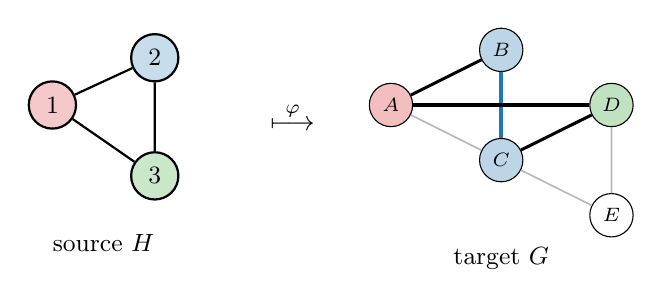
\begin{tikzpicture}[x=1cm,y=1cm,
   lv/.style={circle,draw,thick,minimum size=6mm,inner sep=0pt,font=\small},
   qb/.style={circle,draw,minimum size=5.5mm,inner sep=0pt,font=\scriptsize},
   cpl/.style={gray!55,line width=0.6pt}]
%% ---- source H (triangle 1-2-3) ----
\node[lv,fill=chA!25] (s1) at (0,1.4) {$1$};
\node[lv,fill=chB!25] (s2) at (1.3,2.0) {$2$};
\node[lv,fill=chC!25] (s3) at (1.3,0.5) {$3$};
\draw[thick] (s1)--(s2) (s2)--(s3) (s1)--(s3);
\node at (0.65,-0.35) {\small source $H$};

%% ---- arrow ----
\node at (3.05,1.25) {$\overset{\varphi}{\longmapsto}$};

%% ---- target G with chains ----
\begin{scope}[xshift=4.3cm]
  \node[qb,fill=chA!30] (A) at (0,1.4) {$A$};
  \node[qb,fill=chB!30] (B) at (1.4,2.1) {$B$};
  \node[qb,fill=chB!30] (C) at (1.4,0.7) {$C$};
  \node[qb,fill=chC!30] (D) at (2.8,1.4) {$D$};
  \node[qb] (E) at (2.8,0.0) {$E$};
  % couplers (all light); realized/intra-chain drawn darker
  \draw[cpl] (A)--(C) (C)--(E) (D)--(E);
  \draw[chB,line width=1.4pt] (B)--(C); % intra-chain phi(2)
  \draw[line width=1.1pt] (A)--(B); % H-edge 1-2
  \draw[line width=1.1pt] (C)--(D); % H-edge 2-3
  \draw[line width=1.1pt] (A)--(D); % H-edge 1-3
  \node at (1.4,-0.55) {\small target $G$};
\end{scope}
\end{tikzpicture}
\caption{Minor embedding of the triangle $H$ into a hardware patch $G$.
Vertex $1\!\mapsto\!\varphi(1)=\{A\}$, $2\!\mapsto\!\{B,C\}$,
$3\!\mapsto\!\{D\}$ (matching colours). Chain $\varphi(2)$ is connected through
the bold intra-chain coupler $B\!-\!C$; the three chains are disjoint; each
$H$-edge is realized by a hardware coupler between the corresponding chains
($1\!-\!2$ by $A\!-\!B$, $2\!-\!3$ by $C\!-\!D$, $1\!-\!3$ by $A\!-\!D$). Qubit
$E$ is unused. Here $\mathrm{ACL}=\tfrac{1+2+1}{3}=\tfrac{4}{3}$.}
\label{fig:embedding}
\end{figure}

\paragraph{Contribution.}
This paper makes seven contributions, listed in the order they appear.
(i) We frame minor-embedding chain construction as \emph{multi-net global
routing} and transfer two ideas from FPGA/VLSI computer-aided design---a real
Steiner-tree inner step and \emph{negotiated congestion}---to the
quantum-annealing setting, packaging them as \textbf{Reweave}, an anytime,
large-neighbourhood \emph{improver} that warm-starts from a fast base embedding
and, by construction, never regresses below it (\S\ref{sec:reweave}).
(ii) We evaluate Reweave inside the Ember benchmarking framework
(\S\ref{sec:ember}) against \texttt{minorminer} and
\texttt{minorminer}-with-p-norm-layout on clean and broken Pegasus and on Zephyr
(\S\ref{sec:results}), showing it reduces mean ACL and---the property that most
distinguishes it---run-to-run ACL \emph{variance} in nearly every cell, while all
methods retain full success and validity.
(iii) We \emph{optimize} the algorithm (\S\ref{sec:optimizations}): a structured
pass yields three quality-safe improvements---bounded-region routing, a dirty-set
incremental schedule, and a spur-pruning finishing pass---that together make the
production algorithm ${\sim}3\times$ faster at equal-or-better ACL, within
${\sim}1.3\times$ compiled \texttt{minorminer}'s wall-clock.
(iv) We ask whether \emph{learning} helps (\S\ref{sec:learning}) and report an
honest, cautionary answer: the naive supervised model is ill-posed and collapses,
a symmetry-invariant (Procrustes) objective fixes it and beats \texttt{minorminer}
by ${\sim}1\%$ at equal budget (small but significant), decode-aware RL does not
exceed it, and we retract an earlier unequal-budget comparison.
(v) We open \texttt{minorminer}'s \emph{search order}
(\S\ref{sec:searchguide}) with a ${\sim}90$-line fork that injects a vertex order
into its full search: a Cuthill--McKee order, or a per-instance portfolio, lowers
its ACL by up to ${\sim}5\%$ and roughly halves its variance, composes with Reweave
(the cheap stack \texttt{reweave-mmfork-cuthill}), and stays as reliable as
\texttt{minorminer}---while the complementary rip-up-order lever is inert.
(vi) We study \emph{scaling} on the actual hardware graphs
(\S\ref{sec:scaling})---Advantage Pegasus-$16$ and Advantage2 Zephyr-$15$---and
find the order-guided variants' wall-clock premium \emph{shrinks} with problem
size, running at or below \texttt{minorminer}'s time on the largest instances.
(vii) We \emph{validate} the objective and harden the statistics
(\S\ref{sec:solquality},~\S\ref{sec:rigor}): on a simulator, shorter-chain
embeddings yield significantly better annealing solutions (Spearman $\rho=-0.63$
between ACL and ground-state probability, agreed by simulated annealing and
spin-vector Monte Carlo), and a $K{=}15$-instance redesign with confidence intervals
and paired significance tests confirms the gains and the variance reduction---and
shows which one variant does not survive the stronger design.
Throughout we are explicit (\S\ref{sec:novelty}) that the algorithmic primitives
are not new; the novelty is their synthesis and application to minor embedding,
together with the empirical findings.

%% ========================================================================
\section{Background and Related Work}
\label{sec:related}

\paragraph{The standard heuristic and its weaknesses.}
\texttt{minorminer} (MM), the Cai--Macready--Roy heuristic~\cite{cai2014minorminer},
is randomized coordinate descent. It fixes a random vertex order and, for each
vertex, rips out its chain and rebuilds it as the union of weighted
shortest-path computations to its already-placed neighbours; qubit contention is
discouraged by a vertex weight $\mathrm{diam}(G)^{k}$ where $k$ is the number of
chains currently using the qubit, recomputed from scratch each pass; it iterates
until the embedding is valid or a patience bound is hit. Three structural
weaknesses follow directly. First, a chain is a \emph{union of independent
shortest paths}---a weak Steiner-tree heuristic that misses shared structure.
Second, the congestion signal is \emph{myopic}: a per-pass snapshot with no
memory of how contested a qubit has been over time. Third, the result is highly
\emph{order- and seed-dependent}. The most recent state-of-the-art
evaluation~\cite{gomez2025eval} documents the consequences on broken Pegasus:
run-to-run ACL can differ by several qubits per chain on the same instance, MM is
beaten by deterministic clique embedding once the source's average degree
exceeds the hardware degree, and MM routinely hits a $\sim$1000\,s cutoff on
large dense instances. The MM paper itself names ``better initial placement of
vertex-models'' as the key open problem.

\paragraph{Deterministic templates.}
For sufficiently structured inputs, embeddings can be read off a template.
Clique (``busclique'') embedding generates complete-graph minors in Chimera and
Pegasus connectivity directly~\cite{boothby2016clique}; complete-bipartite
templates~\cite{sinno2025bipartite} and the 4-clique network on a contracted
hardware graph~\cite{pelofske2024fourclique} extend the idea. These are fast and
uniform but over-provision qubits on graphs that are not near-complete.

\paragraph{Layout- and spring-seeded heuristics.}
A complementary line attacks MM's initial-placement weakness by first laying out
the source graph in a low-dimensional space and placing variables near the
geometrically closest qubits: layout-aware embedding~\cite{pinilla2019layout},
the spring/clique-seeded methods of Zbinden et al.~\cite{zbinden2020embedding},
and Ocean's ``Layout Embedding'', which seeds MM with a $p$-norm layout. We use
the latter as a baseline.

\paragraph{Exact methods.}
Integer-programming formulations with Benders
decomposition~\cite{bernal2020ip} and algebraic-geometry/Gr\"obner-basis
compilers~\cite{dridi2018algebraic} solve minor embedding optimally but do not
scale past tens of vertices.

\paragraph{Metaheuristics and learned policies.}
Path/super-vertex simulated annealing (PSSA)~\cite{sugie2018pssa} and
graph-theoretic OCT/virtual-hardware methods~\cite{goodrich2018oct} apply local
search; more recently, GNN-RL (CHARME~\cite{ngo2024charme}) and PPO
policies~\cite{nembrini2025ppo} learn chain-construction heuristics.

\paragraph{Routing and optimal transport.}
Two threads inform our approach. Negotiated-congestion routing
(PathFinder)~\cite{mcmurchie1995pathfinder} from FPGA CAD treats each net as a
resource consumer that negotiates for congested wires over iterations; and
Gromov--Wasserstein optimal transport~\cite{xu2019gwl,vincentcuaz2022srgw}
matches graphs by their intra-graph distances, suggesting a global, continuous
view of the assignment. Our method develops the first thread; the second is
promising future work (\S\ref{sec:limitations}).

%% ========================================================================
\section{The Preliminary Reweave Algorithm}
\label{sec:reweave}

This section presents Reweave as first designed; \S\ref{sec:results} reports
its results. A subsequent optimization pass (\S\ref{sec:optimizations}) makes the
production algorithm $\sim$3$\times$ faster at equal-or-better quality without
changing the ideas below, so we keep this preliminary description intact and
report the optimized numbers separately.

\subsection{Minor embedding as multi-net routing}
A chain $\varphi(v)$ that must be connected and adjacent to each neighbour's
chain is exactly a \emph{Steiner tree} (a routing ``net'') whose terminals are
the qubits bordering the neighbour chains, and the disjointness requirement is
exactly the rule that two nets may not share a routing resource. Minor embedding
is therefore a multi-net global routing problem on the graph $G$, and the
mature machinery of FPGA/VLSI routing applies. We import its two central ideas.

\subsection{A real Steiner inner step}
\label{sec:steiner}
Rather than build a chain as a union of independent shortest paths to a single
root (MM), we grow one tree with the classical \emph{shortest-path heuristic}
(SPH)~\cite{takahashi1980sph,mehlhorn1988steiner}: starting from a root, each
neighbour terminal is connected to the \emph{nearest node of the current tree},
so later connections reuse earlier structure. Figure~\ref{fig:steiner}
contrasts the two: when neighbours cluster, SPH shares a trunk and produces a
strictly shorter chain.

\begin{figure}[t]
\centering
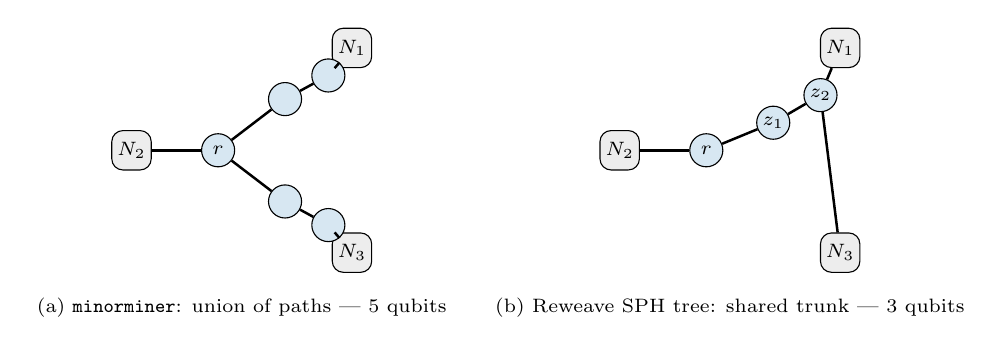
\begin{tikzpicture}[x=1cm,y=1cm,font=\scriptsize,
   q/.style={circle,draw,fill=chB!18,minimum size=4.2mm,inner sep=0pt},
   nb/.style={rounded corners,draw,fill=gray!14,minimum height=5mm,inner sep=2pt},
   e/.style={line width=0.9pt}]
%% ---- panel (a): MM union of shortest paths ----
\begin{scope}
  \node[nb] (N2a) at (-1.1,0) {$N_2$};
  \node[nb] (N1a) at (1.7,1.3) {$N_1$};
  \node[nb] (N3a) at (1.7,-1.3) {$N_3$};
  \node[q] (r) at (0,0) {$r$};
  \node[q] (x1) at (0.85,0.65) {};
  \node[q] (x2) at (1.4,0.95) {};   % path to N1
  \node[q] (y1) at (0.85,-0.65) {};
  \node[q] (y2) at (1.4,-0.95) {};  % path to N3
  \draw[e] (r)--(N2a);
  \draw[e] (r)--(x1)--(x2)--(N1a);
  \draw[e] (r)--(y1)--(y2)--(N3a);
  \node at (0.3,-2.0) {(a) \texttt{minorminer}: union of paths --- $5$ qubits};
\end{scope}
%% ---- panel (b): SPH shared tree ----
\begin{scope}[xshift=6.2cm]
  \node[nb] (N2b) at (-1.1,0) {$N_2$};
  \node[nb] (N1b) at (1.7,1.3) {$N_1$};
  \node[nb] (N3b) at (1.7,-1.3) {$N_3$};
  \node[q] (R) at (0,0) {$r$};
  \node[q] (z1) at (0.85,0.35) {$z_1$};
  \node[q] (z2) at (1.45,0.7) {$z_2$};   % trunk reaching N1
  \draw[e] (R)--(N2b);
  \draw[e] (R)--(z1)--(z2)--(N1b);
  \draw[e] (z2)--(N3b);             % N3 attaches to nearest tree node z2
  \node at (0.3,-2.0) {(b) Reweave SPH tree: shared trunk --- $3$ qubits};
\end{scope}
\end{tikzpicture}
\caption{Inner step contrast for a chain that must reach three neighbour chains
$N_1,N_2,N_3$. (a) MM routes an independent shortest path to each, duplicating
qubits when $N_1$ and $N_3$ are near each other. (b) The shortest-path-heuristic
Steiner tree attaches $N_3$ to the nearest existing tree node ($z_2$), reusing
the trunk built for $N_1$, yielding a shorter chain.}
\label{fig:steiner}
\end{figure}

\subsection{Negotiated congestion}
\label{sec:negotiation}
We replace MM's snapshot penalty with the negotiated-congestion cost of
McMurchie and Ebeling~\cite{mcmurchie1995pathfinder}. Routing prices each qubit
$q$ at
\begin{equation}
  \mathrm{cost}(q) \;=\; \bigl(1 + h_q\bigr)\,\bigl(1 + \lambda \cdot o_q\bigr),
  \label{eq:cost}
\end{equation}
where $o_q$ is the number of \emph{other} chains currently occupying $q$
(occupancy), $\lambda$ is the present-congestion factor, and $h_q$ is a
\emph{history} term that \emph{accumulates} by a fixed increment every iteration
in which $q$ is over-subscribed. The present term makes a qubit more expensive as
nets pile onto it within a pass; the history term gives the price a memory, so a
persistently contested qubit becomes permanently expensive and the chains that
can most cheaply route around it eventually yield. This is a Lagrangian view of
the disjointness constraint; in FPGA routing it is known to drive the search
toward a legal, low-congestion state, and we observe the same behaviour
here---behaviour MM's memoryless snapshot cannot sustain. A
node-weighted Dijkstra over Eq.~\eqref{eq:cost} supplies the shortest-path
computations the SPH step needs.

\subsection{A warm-started large-neighbourhood improver}
\label{sec:improver}
A from-scratch router that places every chain from scattered single-qubit seeds
is throttled by exactly the open problem MM names---\emph{initial placement}.
Without co-locating adjacent variables, dense-graph chains balloon and the search
often fails to legalize at all. The standalone \texttt{reweave-cold} variant
(a cold start followed by the same improver) bears this out: on the nine
clean-Pegasus Erd\H{o}s--R\'enyi instances of our grid
($n\in\{20,30,40\}$, $d\in\{0.3,0.5,0.7\}$) it legalizes only four---the smaller
and sparser ones, at ACL $2.5$--$3.8$---and fails on the five larger, denser ones,
whereas
\texttt{minorminer} embeds all nine
(reproduced by \texttt{docs/paper/data/coldstart\_probe.py}).
Reweave therefore runs as an \emph{improver}. It warm-starts from a fast base
embedding (MM by default; any registered algorithm works), then performs
\emph{large-neighbourhood} rip-up-and-reroute---the neighbourhood being a long
chain together with the cascade of chains its rerouting displaces. It takes the
longest chain and lets it re-route along the cheapest tree under
Eq.~\eqref{eq:cost}---which may cross occupied territory and create temporary
overlaps---then re-routes every chain it displaced through free space. A move is
committed only if it lowers the embedding's total qubit count (equivalently, its
ACL) and leaves it valid; otherwise the prior state is restored
(Algorithms~\ref{alg:driver}--\ref{alg:move}). Because Reweave keeps the best
valid embedding it has seen, it \textbf{never returns an embedding worse than its
base}, and it spends its entire time budget reducing ACL---an anytime guarantee
MM's one-shot, patience-bounded run lacks. The \texttt{thorough} configuration
additionally runs four seeded restarts and keeps the best, trading wall-clock for
lower ACL and variance. When no valid base is available, a fallback builds the
initial embedding from scratch in breadth-first vertex order under the same
negotiated cost; uncompetitive on its own, it exists only to guarantee an output.

\begin{algorithm}[t]
\caption{Reweave (driver)}
\label{alg:driver}
\begin{algorithmic}[1]
\Require source $H$, target $G$, base embedder $\mathcal{B}$
\State $\Phi \gets \mathcal{B}(H,G)$ \Comment{warm start}
\If{$\Phi$ invalid} $\Phi \gets \textsc{ColdStart}(H,G)$ \Comment{BFS-ordered negotiated fallback}
\EndIf
\If{$\Phi$ invalid} \Return failure \EndIf
\State $\Phi^\star \gets \Phi$ \Comment{best valid so far}
\Repeat
  \ForAll{$v \in V(H)$ in decreasing chain length}
     \State $\Phi \gets \textsc{TryShorten}(\Phi, v)$ \Comment{Alg.~\ref{alg:move}}
     \If{$\mathrm{ACL}(\Phi) < \mathrm{ACL}(\Phi^\star)$} $\Phi^\star \gets \Phi$ \EndIf
  \EndFor
\Until{no improvement \textbf{or} deadline}
\State \Return $\Phi^\star$
\end{algorithmic}
\end{algorithm}

\begin{algorithm}[t]
\caption{\textsc{TryShorten}$(\Phi, v)$ --- one LNS destroy-repair move}
\label{alg:move}
\begin{algorithmic}[1]
\State snapshot $\Phi$
\State rip up $\varphi(v)$; rebuild it as the cheapest SPH tree under
       Eq.~\eqref{eq:cost} \Comment{may overlap others}
\If{new chain not shorter} restore; \Return $\Phi$ \EndIf
\ForAll{chain $w$ now overlapping $\varphi(v)$}
   \State rip up $\varphi(w)$; reroute it through free qubits only
   \If{no free-space route} restore; \Return $\Phi$ \EndIf
\EndFor
\If{total qubits decreased \textbf{and} $\Phi$ valid} \Return $\Phi$
\Else{} restore; \Return $\Phi$ \EndIf
\end{algorithmic}
\end{algorithm}

\subsection{Novelty}
\label{sec:novelty}
We state plainly what is and is not new. Negotiated-congestion routing is due to
McMurchie and Ebeling~\cite{mcmurchie1995pathfinder}; the shortest-path Steiner
heuristic is classical~\cite{takahashi1980sph,mehlhorn1988steiner}; and
large-neighbourhood/destroy-repair search is a standard matheuristic paradigm.
\emph{None of these primitives is our invention.} The contribution is their
synthesis and their application to quantum-annealing minor embedding: casting
chain construction as multi-net routing, replacing MM's two weakest components
(its inner step and its congestion signal) in a single drop-in algorithm,
running it as a warm-started anytime improver with a never-regress guarantee, and
validating empirically that this reduces ACL and---more importantly---ACL
variance against the standard tool. The clean substitution also isolates a
question of independent interest: \emph{is it MM's congestion signal or its
inner step that costs the most?}

%% ========================================================================
\section{Ember and Evaluation Methodology}
\label{sec:ember}

We evaluate inside \textbf{Ember} (\texttt{ember-qc}), an open benchmarking
framework for minor-embedding algorithms on D-Wave topologies. Every algorithm
implements a common interface and is run through Ember's atomic harness
\texttt{benchmark\_one}, which times the call and computes quality metrics
(chain lengths, ACL, max chain length, qubits, couplers). Before any metric is
trusted, the output passes four-layer validation: type and format checks
followed by the structural checks of \S\ref{sec:intro} (coverage, connectivity,
disjointness, edge preservation). Targets are generated with
\texttt{dwave-networkx} and may have qubits removed to simulate fabrication
faults, and per-trial seeds are derived deterministically by SHA-256 of the task
identity, so runs are reproducible and order-independent. Results aggregate into
per-group means and standard deviations.

\paragraph{Protocol.}
Targets are clean Pegasus~$P_6$, a \emph{broken} Pegasus~$P_6$ with $5\%$ of
qubits removed at random (the state-of-the-art evaluation setting), and
Zephyr~$Z_4$. Sources are an Erd\H{o}s--R\'enyi (ER) grid over
$n\in\{20,30,40\}$ and edge density $d\in\{0.3,0.5,0.7\}$, plus $d$-regular and
Barab\'asi--Albert graphs for generality; one fixed instance per cell, so the
reported spread is the run-to-run variance \emph{on a fixed instance}---MM's
documented failure mode. Baselines are \texttt{minorminer} and
\texttt{minorminer-layout} ($p$-norm layout). Each (algorithm, instance) is run
over five seeds; we report success rate, ACL mean and standard deviation, max
chain length, qubits, and wall-clock time.

%% ========================================================================
\section{Preliminary Results}
\label{sec:results}

These are the results of the preliminary algorithm of \S\ref{sec:reweave};
the optimized production version and its (improved, and much faster) numbers
follow in \S\ref{sec:optimizations}. All four methods embed every instance across
all seeds and topologies ($100\%$ success), so success is not a differentiator on
this grid; the
comparison is on chain length, its variance, and time. Table~\ref{tab:quality}
reports embedding quality on clean Pegasus~$P_6$, Table~\ref{tab:timing} the
corresponding wall-clock time, and Table~\ref{tab:robust} robustness across
topologies; Figure~\ref{fig:density} shows the density trend.

Two findings are sharp. First, the single-seed \texttt{reweave} \emph{never
regresses}: across all $35$ instance--topology cells (every per-seed run, in
fact) its mean ACL is $\le$ \texttt{minorminer}'s---the maximum observed
difference is $0.000$ to three decimals---confirming the best-valid guarantee
empirically. Second, \texttt{reweave-thorough} lowers mean ACL on the six
shown cells by $3.2$--$4.5\%$, and reduces ACL standard deviation in five of the
six---by up to $76\%$ on the full clean-$P_6$ grid (e.g.\
$0.11\!\to\!0.03$ at $n{=}30,d{=}0.3$). The lone clean-$P_6$ exception is
$n{=}40,d{=}0.3$, where \texttt{minorminer}'s spread is already at the floor
($0.05$); we report it rather than hide it. The complete $35$-cell grid across
all three source families is in Appendix~\ref{app:full}: there
\texttt{reweave-thorough} lowers mean ACL on \emph{every} cell (by
$1$--$11\%$; the largest single gain, $-10.6\%$, is on a $d$-regular source) and
cuts ACL standard deviation in $30$ of the $35$.

\begin{table}[t]
\caption{Embedding quality on clean Pegasus~$P_6$ for ER sources (mean over $5$
seeds; ACL std in parentheses; lower ACL is better). Best ACL per cell in bold.}
\label{tab:quality}
\small
\begin{tabular}{llccc}
\toprule
cell & algorithm & ACL (std) & max & qubits \\
\midrule
\multirow{4}{*}{$n{=}30,d{=}0.3$}
 & \texttt{minorminer}          & 2.70 (0.11) & 3.8 & 81.0 \\
 & \texttt{minorminer-layout}   & 2.75 (0.15) & 4.0 & 82.4 \\
 & \texttt{reweave}          & 2.69 (0.10) & 3.8 & 80.6 \\
 & \texttt{reweave-thorough} & \textbf{2.59} (0.03) & 3.8 & 77.6 \\
\midrule
\multirow{4}{*}{$n{=}30,d{=}0.5$}
 & \texttt{minorminer}          & 3.30 (0.16) & 4.6 & 99.0 \\
 & \texttt{minorminer-layout}   & 3.43 (0.10) & 4.8 & 102.8 \\
 & \texttt{reweave}          & 3.25 (0.15) & 4.6 & 97.6 \\
 & \texttt{reweave-thorough} & \textbf{3.19} (0.10) & 4.0 & 95.8 \\
\midrule
\multirow{4}{*}{$n{=}30,d{=}0.7$}
 & \texttt{minorminer}          & 3.83 (0.22) & 5.0 & 114.8 \\
 & \texttt{minorminer-layout}   & 3.80 (0.17) & 5.4 & 114.0 \\
 & \texttt{reweave}          & 3.79 (0.23) & 5.0 & 113.8 \\
 & \texttt{reweave-thorough} & \textbf{3.65} (0.06) & 4.8 & 109.6 \\
\midrule
\multirow{4}{*}{$n{=}40,d{=}0.3$}
 & \texttt{minorminer}          & 3.56 (0.05) & 5.2 & 142.4 \\
 & \texttt{minorminer-layout}   & 3.62 (0.14) & 5.4 & 144.8 \\
 & \texttt{reweave}          & 3.53 (0.06) & 5.2 & 141.0 \\
 & \texttt{reweave-thorough} & \textbf{3.41} (0.06) & 5.0 & 136.4 \\
\midrule
\multirow{4}{*}{$n{=}40,d{=}0.5$}
 & \texttt{minorminer}          & 4.57 (0.10) & 6.4 & 182.6 \\
 & \texttt{minorminer-layout}   & 4.72 (0.13) & 6.8 & 188.8 \\
 & \texttt{reweave}          & 4.49 (0.14) & 6.2 & 179.6 \\
 & \texttt{reweave-thorough} & \textbf{4.39} (0.08) & 6.2 & 175.4 \\
\midrule
\multirow{4}{*}{$n{=}40,d{=}0.7$}
 & \texttt{minorminer}          & 5.15 (0.06) & 7.2 & 206.0 \\
 & \texttt{minorminer-layout}   & 5.23 (0.17) & 7.0 & 209.2 \\
 & \texttt{reweave}          & 5.07 (0.04) & 7.0 & 202.6 \\
 & \texttt{reweave-thorough} & \textbf{4.98} (0.04) & 7.0 & 199.0 \\
\bottomrule
\end{tabular}
\end{table}

\begin{table}[t]
\caption{Wall-clock time (mean seconds per embedding, clean $P_6$). Reweave
is pure Python; \texttt{minorminer} is compiled C++. \texttt{reweave-thorough}
runs four seeded restarts and may use up to the full $20$\,s time budget.}
\label{tab:timing}
\small
\begin{tabular}{lrrrr}
\toprule
cell & \texttt{mm} & \texttt{mm-layout} & \texttt{rw} & \texttt{rw-thor.} \\
\midrule
$n{=}30,d{=}0.3$ & 0.33 & 0.33 & 1.11 & 20.08 \\
$n{=}30,d{=}0.5$ & 4.44 & 3.30 & 9.04 & 18.82 \\
$n{=}30,d{=}0.7$ & 1.22 & 0.98 & 3.23 & 12.33 \\
$n{=}40,d{=}0.3$ & 0.54 & 0.46 & 2.12 & 8.37 \\
$n{=}40,d{=}0.5$ & 1.11 & 0.99 & 4.12 & 16.41 \\
$n{=}40,d{=}0.7$ & 1.35 & 1.73 & 5.87 & 20.01 \\
\bottomrule
\end{tabular}
\end{table}

\begin{table}[t]
\caption{Robustness across topologies for the $n{=}40,d{=}0.5$ ER source: ACL
(std) and time. \texttt{minorminer}'s ACL inflates most on broken Pegasus, where
\texttt{reweave-thorough}'s relative gain is largest ($-7.3\%$).}
\label{tab:robust}
\small
\begin{tabular}{llcc}
\toprule
target & algorithm & ACL (std) & time (s) \\
\midrule
\multirow{4}{*}{Pegasus $P_6$}
 & \texttt{minorminer}          & 4.57 (0.10) & 1.11 \\
 & \texttt{minorminer-layout}   & 4.72 (0.13) & 0.99 \\
 & \texttt{reweave}          & 4.49 (0.14) & 4.12 \\
 & \texttt{reweave-thorough} & \textbf{4.39} (0.08) & 16.41 \\
\midrule
\multirow{4}{*}{broken $P_6$ ($5\%$)}
 & \texttt{minorminer}          & 4.88 (0.18) & 0.82 \\
 & \texttt{minorminer-layout}   & 4.72 (0.19) & 1.19 \\
 & \texttt{reweave}          & 4.80 (0.18) & 3.52 \\
 & \texttt{reweave-thorough} & \textbf{4.52} (0.06) & 14.26 \\
\midrule
\multirow{4}{*}{Zephyr $Z_4$}
 & \texttt{minorminer}          & 3.63 (0.08) & 0.98 \\
 & \texttt{minorminer-layout}   & 3.61 (0.16) & 1.10 \\
 & \texttt{reweave}          & 3.57 (0.07) & 3.81 \\
 & \texttt{reweave-thorough} & \textbf{3.52} (0.03) & 13.90 \\
\bottomrule
\end{tabular}
\end{table}

\begin{figure}[t]
\centering
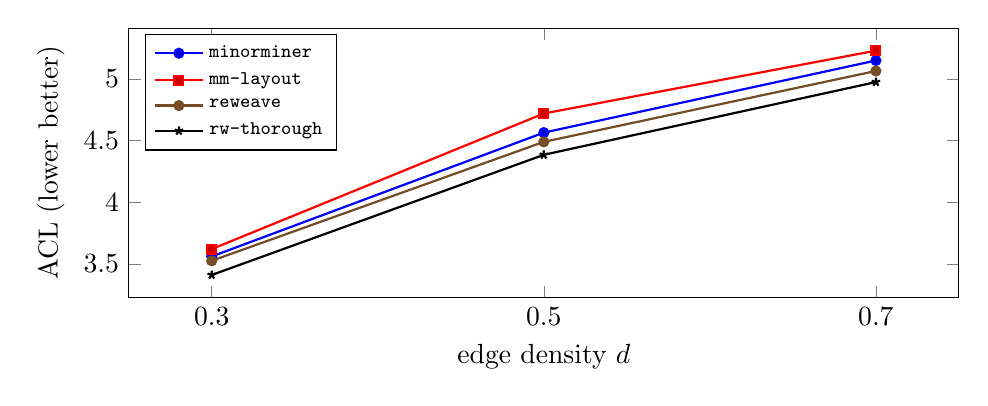
\begin{tikzpicture}
\begin{axis}[
  width=\columnwidth, height=5cm,
  xlabel={edge density $d$}, ylabel={ACL (lower better)},
  xtick={0.3,0.5,0.7}, xmin=0.25, xmax=0.75,
  legend style={font=\scriptsize, at={(0.02,0.98)}, anchor=north west},
  legend cell align=left, mark size=1.6pt,
]
\addplot+[thick] coordinates {(0.3,3.56)(0.5,4.565)(0.7,5.15)};
\addplot+[thick] coordinates {(0.3,3.62)(0.5,4.72)(0.7,5.23)};
\addplot+[thick] coordinates {(0.3,3.525)(0.5,4.49)(0.7,5.065)};
\addplot+[thick] coordinates {(0.3,3.41)(0.5,4.385)(0.7,4.975)};
\legend{\texttt{minorminer}, \texttt{mm-layout}, \texttt{reweave}, \texttt{rw-thorough}}
\end{axis}
\end{tikzpicture}
\caption{ACL versus edge density for $n{=}40$ ER sources on clean Pegasus~$P_6$.
\texttt{reweave-thorough} (bottom curve) is uniformly shortest; the gap to
\texttt{minorminer} is roughly constant in absolute terms across densities.}
\label{fig:density}
\end{figure}

\paragraph{Discussion.}
The single-seed \texttt{reweave} is the fair \emph{equal-base} comparison: it
consumes the same \texttt{minorminer} base for a given seed and only refines it,
so it cannot regress---and it already trims ACL on denser cells while leaving the
sparse and $d$-regular cells (where the base is near-optimal) unchanged. The
substantive gains come from \texttt{reweave-thorough}, whose four restarts
both lower the mean and, by selecting the best of several runs, sharply cut the
run-to-run variance that is \texttt{minorminer}'s signature weakness. The effect
persists on broken Pegasus---where \texttt{minorminer}'s ACL inflates most and the
thorough gain is largest---and on Zephyr, so the mechanism is not
topology-specific. The cost is wall-clock time: Reweave layers a pure-Python
router on top of the base, and \texttt{reweave-thorough}, with its four
restarts, can use the full $20$\,s budget; \texttt{minorminer-layout}, by
contrast, is neither consistently faster nor consistently better than plain
\texttt{minorminer}.

%% ========================================================================
\section{Optimizations}
\label{sec:optimizations}

The preliminary algorithm wins on chain length and variance but pays in
wall-clock: its pure-Python router is $\sim$3--6$\times$ slower than compiled
\texttt{minorminer} (Table~\ref{tab:timing}). We therefore ran a structured
optimization pass---eight candidate improvements (five targeting speed, three
quality), each implemented as an isolated variant and measured against the frozen
preliminary algorithm. Three quality-safe winners survived and are baked into the
production algorithm; the rest were rejected or deferred.

\paragraph{What we bake in.} The three production optimizations are mutually
orthogonal (each rewrites a different stage of the router) and compose without
interaction:
\begin{itemize}
  \item \textbf{Bounded-region routing.} Each per-neighbour shortest-path search
    is restricted to a breadth-first ball around the vertex's current chain and
    its placed-neighbour chains, and stops as soon as the neighbour boundary is
    settled, instead of computing a full single-source shortest-path tree over
    the whole 680--5640-qubit fabric. Alone this is $\sim$3$\times$ faster with
    byte-identical chains.
  \item \textbf{Dirty-set incremental scheduling.} The improvement loop keeps a
    worklist of vertices whose neighbourhood changed rather than re-sweeping
    every chain each round; it performs the same accepted moves with fewer
    wasted re-examinations.
  \item \textbf{Spur-pruning.} A deterministic finishing pass removes redundant
    chain leaves---qubits whose removal keeps the chain connected and breaks no
    incident edge---to a fixpoint. This is the cheap shadow of exact region
    repair: on \texttt{minorminer}'s own output it recovers about half of a
    CP-SAT repair's ACL gain at $\sim$5000$\times$ less time, and on Reweave it
    shaves a further ${\sim}0.6\%$ ACL for free.
\end{itemize}
A fourth idea---seeding the improver from a multilevel placement instead of
\texttt{minorminer}---lowers ACL and variance on large, dense Pegasus instances
(e.g.\ $-6\%$ ACL and $-17\%$ seed std at $n{=}40,d{=}0.7$ under the $K{=}15$ design
of \S\ref{sec:rigor}), but the multilevel base is unreliable on small, sparse, and
Zephyr instances (it inflated ACL by up to $30\%$ where \texttt{minorminer} is already
near-optimal, so that pooled over the grid it is a net regression), so we keep it as
an optional variant rather than the default. We also rejected an A\,$^\star$ routing
scheme (a $+1.7\%$ ACL regression) and an exact Dreyfus--Wagner Steiner inner step
(no gain over the shortest-path heuristic). A compiled (numba) node-weighted
Dijkstra core, which we built and tested, gives \emph{no} net speedup once
bounded-region routing has localized each search
(\S\ref{sec:limitations})---so the production router stays pure Python; only
parallelized restarts remain as future speed work.

\paragraph{Optimized results.} Tables~\ref{tab:optquality} and~\ref{tab:opttime}
report the optimized algorithm on the clean-Pegasus grid. The optimizations are
quality-safe: optimized \texttt{reweave} is never worse than the preliminary
engine and, thanks to spur-pruning, slightly better---mean ACL $-1.3\%$ vs.\
\texttt{minorminer} over all $35$ cells (vs.\ $-0.9\%$ for the preliminary
engine), and $-2.1\%$ vs.\ \texttt{minorminer-layout}. The headline is speed:
single-seed \texttt{reweave} now runs in ${\sim}1.3\times$
\texttt{minorminer}'s wall-clock (down from ${\sim}3$--$5\times$) while producing
shorter chains, and the optimized \texttt{reweave-thorough} delivers $-5.1\%$
mean ACL vs.\ \texttt{minorminer} (up to $-10.6\%$; $-5.9\%$ vs.\ layout) at
roughly the former cost of a \emph{single} preliminary run rather than four. The
optimized Reweave thus keeps the quality advantage of \S\ref{sec:results}
while closing most of the wall-clock gap to compiled \texttt{minorminer}.

\begin{table}[t]
\caption{\textbf{Optimized} Reweave, embedding quality on clean Pegasus~$P_6$
(ER sources, mean over $5$ seeds; ACL std in parentheses; lower is better). Best
ACL per cell in bold. Cf.\ the preliminary Table~\ref{tab:quality}; the optimized
\texttt{reweave} matches-or-beats it everywhere at ${\sim}3\times$ less time
(Table~\ref{tab:opttime}).}
\label{tab:optquality}
\small
\begin{tabular}{llcc}
\toprule
cell & algorithm & ACL (std) & qubits \\
\midrule
\multirow{4}{*}{$n{=}30,d{=}0.3$}
 & \texttt{minorminer}          & 2.70 (0.11) & 81.0 \\
 & \texttt{minorminer-layout}   & 2.75 (0.15) & 82.4 \\
 & \texttt{reweave}          & 2.68 (0.11) & 80.4 \\
 & \texttt{reweave-thorough} & \textbf{2.58} (0.03) & 77.4 \\
\midrule
\multirow{4}{*}{$n{=}30,d{=}0.5$}
 & \texttt{minorminer}          & 3.30 (0.16) & 99.0 \\
 & \texttt{minorminer-layout}   & 3.43 (0.10) & 102.8 \\
 & \texttt{reweave}          & 3.23 (0.15) & 97.0 \\
 & \texttt{reweave-thorough} & \textbf{3.17} (0.11) & 95.0 \\
\midrule
\multirow{4}{*}{$n{=}30,d{=}0.7$}
 & \texttt{minorminer}          & 3.83 (0.22) & 114.8 \\
 & \texttt{minorminer-layout}   & 3.80 (0.17) & 114.0 \\
 & \texttt{reweave}          & 3.77 (0.20) & 113.0 \\
 & \texttt{reweave-thorough} & \textbf{3.65} (0.07) & 109.4 \\
\midrule
\multirow{4}{*}{$n{=}40,d{=}0.3$}
 & \texttt{minorminer}          & 3.56 (0.05) & 142.4 \\
 & \texttt{minorminer-layout}   & 3.62 (0.14) & 144.8 \\
 & \texttt{reweave}          & 3.51 (0.06) & 140.4 \\
 & \texttt{reweave-thorough} & \textbf{3.39} (0.06) & 135.6 \\
\midrule
\multirow{4}{*}{$n{=}40,d{=}0.5$}
 & \texttt{minorminer}          & 4.57 (0.10) & 182.6 \\
 & \texttt{minorminer-layout}   & 4.72 (0.13) & 188.8 \\
 & \texttt{reweave}          & 4.45 (0.11) & 177.8 \\
 & \texttt{reweave-thorough} & \textbf{4.35} (0.08) & 174.0 \\
\midrule
\multirow{4}{*}{$n{=}40,d{=}0.7$}
 & \texttt{minorminer}          & 5.15 (0.06) & 206.0 \\
 & \texttt{minorminer-layout}   & 5.23 (0.17) & 209.2 \\
 & \texttt{reweave}          & 4.95 (0.06) & 198.0 \\
 & \texttt{reweave-thorough} & \textbf{4.87} (0.03) & 194.8 \\
\bottomrule
\end{tabular}
\end{table}

\begin{table}[t]
\caption{Wall-clock after optimization (mean seconds per embedding, clean $P_6$).
``prelim.'' is the preliminary single-seed engine (\texttt{reweave-base}).
Optimized \texttt{reweave} matches \texttt{minorminer} to within ${\sim}1.3\times$
and is ${\sim}3\times$ faster than the preliminary engine; optimized
\texttt{reweave-thorough} (best-of-4) costs about what a single preliminary run
did.}
\label{tab:opttime}
\small
\begin{tabular}{lrrrr}
\toprule
cell & \texttt{mm} & prelim. & \texttt{rw} & \texttt{rw-thor.} \\
\midrule
$n{=}30,d{=}0.3$ & 0.22 & 0.94 & 0.27 & 1.08 \\
$n{=}30,d{=}0.5$ & 0.70 & 2.08 & 0.75 & 2.31 \\
$n{=}30,d{=}0.7$ & 0.83 & 2.82 & 1.03 & 3.41 \\
$n{=}40,d{=}0.3$ & 0.53 & 2.12 & 0.68 & 2.40 \\
$n{=}40,d{=}0.5$ & 1.15 & 3.86 & 1.33 & 5.08 \\
$n{=}40,d{=}0.7$ & 1.33 & 5.59 & 1.87 & 8.41 \\
\bottomrule
\end{tabular}
\end{table}

%% ========================================================================
\section{A Learning-Based Approach}
\label{sec:learning}

Reweave is a hand-engineered improver. A complementary question is whether an
\emph{amortized} model can \emph{learn} to embed---paying an offline training cost
once and then predicting an embedding in a single forward pass, rather than
searching at solve time. This amortized premise---a deep network that accelerates
graph embedding---is precisely that of a recent patent application
\cite{hyde2025dlembedding}. The cache of problems Reweave has already solved is a
ready-made training set---and reusing embeddings cached from previously-solved
problems is itself a patented strategy~\cite{brahm2021caching}: each \emph{(problem
graph, Reweave-optimized embedding)} pair is a labelled example, and we ask a model
to reproduce---and ideally improve on---that quality. This mirrors the
predict-then-refine pattern of learned embedding heuristics
\cite{ngo2024charme,nembrini2025ppo}, where a network proposes a candidate that a
classical minor-embedding step then refines.

We implemented several model families \emph{inside Ember}, so they are benchmarked
through the exact same harness (\S\ref{sec:results}) as \texttt{minorminer} (MM) and
Reweave. The honest finding is a cautionary one with a useful twist. The obvious
supervised approach---regress each vertex's hardware coordinate from a graph-VAE or
GNN---is \textbf{ill-posed and collapses to a constant} (\S\ref{sec:learn-collapse}),
and an early ``the VAE beats Reweave-thorough'' reading was an artifact of an
unequal restart budget, which we retract. The fix is a \textbf{symmetry-invariant
(Procrustes) objective} (\S\ref{sec:learn-fix}) that recovers a real layout and beats
\texttt{minorminer} by ${\sim}1\%$ at equal budget---statistically significant but
small, and a decode-aware reinforcement-learning fine-tune does not exceed it. We
report the whole arc, because the failure mode is as instructive as the fix.

\subsection{Embedding as a learned layout}
\label{sec:learn-layout}

The central reduction is to predict a \emph{layout} rather than an embedding
directly. Every family maps each logical vertex $v$ to a coordinate
$\hat{p}(v)\in[0,1]^2$ in the target's normalized hardware frame (read off the
Pegasus/Zephyr drawing layout). Two decoders turn a layout into a valid embedding,
both reusing Reweave's repair backend (\S\ref{sec:reweave}) so that no
validity logic is re-implemented:
\emph{seed}$\rightarrow$\emph{MM} snaps each vertex to a distinct nearest qubit (an
optimal linear-assignment problem) and hands those single-qubit chains to
\texttt{minorminer} as \texttt{initial\_chains}; \emph{direct}$\rightarrow$%
\emph{repair} forms a proximity soft-assignment and rounds, grows, and legalizes it.
Feeding the \emph{true} Reweave chain centroids through the seed decoder recovers
Reweave-quality embeddings (mean ACL within $1.03\times$, $100\%$ valid), so the
decoder is near-lossless: the learning problem is exactly ``predict a good layout.''

\subsection{Background: variational autoencoders on graphs}

A variational autoencoder (VAE) \cite{kingma2014vae} learns a probabilistic encoder
$q_\phi(z\mid x)$ and decoder $p_\theta(x\mid z)$ over a latent variable $z$,
trained by maximizing the evidence lower bound
\[
  \mathcal{L}(\theta,\phi)=\mathbb{E}_{q_\phi(z\mid x)}\!\left[\log p_\theta(x\mid z)\right]
  -\beta\,\mathrm{KL}\!\left(q_\phi(z\mid x)\,\|\,p(z)\right),
\]
a reconstruction term traded against a standard-normal prior $p(z)$. Graph VAEs
replace the encoder with a graph neural network and have been used to embed and
generate graphs \cite{kipf2016vgae,simonovsky2018graphvae}. Our encoder is a
message-passing GNN (a residual GraphSAGE stack \cite{hamilton2017graphsage}; a
graph-attention encoder \cite{velickovic2018gat} is a drop-in alternative). The
twist is twofold: the decoder emits a hardware \emph{layout} rather than a
reconstructed graph, and we exploit the model's \emph{generative} nature at
inference time---sampling several latents yields several candidate layouts, and we
keep the best after decoding. This is a cheap, learned analogue of
Reweave-thorough's best-of-$N$ restarts. As \S\ref{sec:learn-collapse} shows, for
the \emph{collapsed} VAE this best-of-$K$ wrapper turns out to be the \emph{only}
thing it contributes---which is exactly why an early reading of it as a win was
mistaken.

\subsection{The \texttt{learned-vae} architecture}
\label{sec:learn-arch}

Figure~\ref{fig:vae} sketches the model. The encoder runs a residual GraphSAGE
backbone ($5$ layers, width $160$) over the source graph's structural node features
(degree, clustering, triangle and core numbers, and an $8$-dimensional Laplacian
positional encoding), then pools the node embeddings $h_v$ with concatenated
mean-and-max pooling and projects to a Gaussian posterior $\mathcal{N}(\mu,\sigma^2)$
over a latent of dimension $16$. The decoder concatenates each node embedding $h_v$
with the (broadcast) latent $z$ and maps it through an MLP with a sigmoid head to a
coordinate $\hat{p}(v)\in[0,1]^2$. Training minimizes the ELBO with reconstruction
$\lVert \hat{p}-y\rVert^2$ against the Reweave chain-centroid labels $y$ and a
KL term with $\beta{=}0.01$ (linearly warmed up); the deterministic layout $z{=}\mu$
serves the layout interface used for model selection.

\emph{Inference} is generative: encode the query once, draw $K{=}8$ latents
$z^{(1)}{=}\mu, z^{(2)},\dots,z^{(K)}\sim\mathcal{N}(\mu,\sigma^2)$, decode each to a
layout, run the seed$\rightarrow$MM decoder on each, and return the lowest-ACL valid
embedding. The $K$ decode passes share the encode and are individually fast; the
per-sample \texttt{minorminer} budget is apportioned so the total stays within the
wall-clock budget.

\begin{figure}[t]
\centering
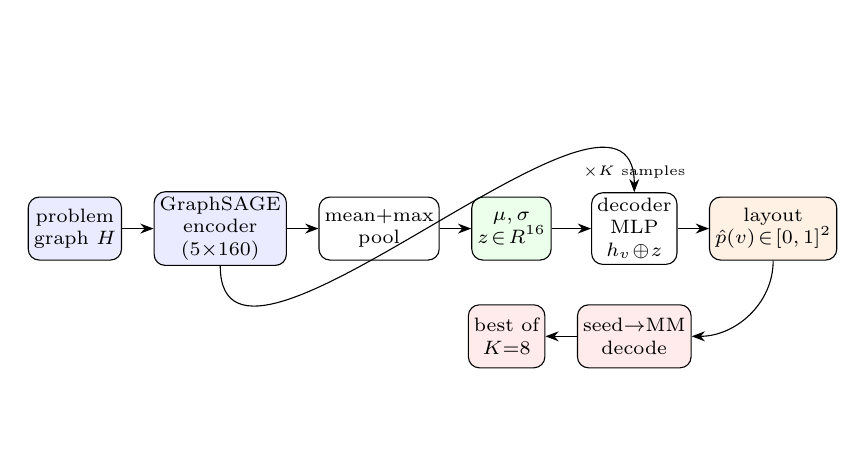
\begin{tikzpicture}[font=\scriptsize,
  box/.style={draw,rounded corners,minimum height=8mm,align=center,inner sep=2pt},
  >=Stealth]
\node[box,fill=blue!8] (h) {problem\\graph $H$};
\node[box,right=4mm of h,fill=blue!8] (gnn) {GraphSAGE\\encoder\\($5{\times}160$)};
\node[box,right=4mm of gnn] (pool) {mean$+$max\\pool};
\node[box,right=4mm of pool,fill=green!8] (z) {$\mu,\sigma$\\$z\!\in\!\mathbb{R}^{16}$};
\node[box,right=5mm of z] (dec) {decoder\\MLP\\$h_v\!\oplus\!z$};
\node[box,right=4mm of dec,fill=orange!10] (lay) {layout\\$\hat p(v)\!\in\![0,1]^2$};
\node[box,below=5mm of dec,fill=red!8] (mm) {seed$\to$MM\\decode};
\node[box,left=4mm of mm,fill=red!8] (best) {best of\\$K{=}8$};
\draw[->] (h)--(gnn); \draw[->] (gnn)--(pool); \draw[->] (pool)--(z);
\draw[->] (z)--(dec); \draw[->] (dec)--(lay);
\draw[->] (gnn.south) to[out=-90,in=90] (dec.north);
\draw[->] (lay) to[out=-90,in=0] (mm);
\draw[->] (mm)--(best);
\node[above=0.5mm of dec,font=\tiny] {$\times K$ samples};
\end{tikzpicture}
\caption{\texttt{learned-vae}. A graph-VAE encodes $H$ to a latent $z$; the decoder
turns $z$ (plus per-node features) into a hardware \emph{layout}; $K{=}8$ sampled
layouts are each decoded to a valid embedding via seed$\to$\texttt{minorminer}, and
the shortest-ACL one is returned.}
\label{fig:vae}
\end{figure}

\subsection{Dataset generation}
\label{sec:learn-data}

Supervision comes entirely from Reweave, so the corpus must be diverse and the
splits clean. We sample source graphs from four families across a size grid
$n\in\{10,\dots,50\}$: Erd\H{o}s--R\'enyi $G(n,p)$, random $d$-regular,
Barab\'asi--Albert, and $k$-nearest-neighbour geometric graphs, over a grid of the
relevant density/degree/radius parameter. Each graph is labelled by running
\texttt{reweave-thorough} through Ember's \texttt{benchmark\_one} into both
clean Pegasus $P_6$ ($680$ qubits) and Zephyr $Z_4$ ($576$ qubits); only graphs it
validly embeds contribute a label for that target. The supervised target for vertex
$v$ is the centroid, in normalized hardware coordinates, of its Reweave chain.

Splits are \textbf{instance-disjoint}: train, validation, and test draw from
disjoint random-seed ranges \emph{per grid cell}, so a graph (and its isomorphs from
the same generator seed) can never appear in two splits---the property reviewers of
learned combinatorial solvers rightly scrutinize. The realized corpus is $1560$
train, $312$ validation, and $312$ test graphs, i.e.\ $3120/624/624$ labelled
(graph, target, embedding) examples after the both-target labelling. Generation is
deterministic (seeded) and embarrassingly parallel; the full corpus labels in a few
minutes across a multi-core node.

\subsection{Training}
\label{sec:learn-train}

Models are trained with Adam \cite{kingma2015adam} (learning rate $2{\times}10^{-3}$,
cosine decay, batch size $16$) and---crucially---\textbf{selected on the real
downstream metric}: every few epochs we decode the validation layouts through
seed$\rightarrow$MM and keep the checkpoint with the best validation ACL ratio, not
the one with the lowest loss. Training is cheap: the $P_6$ \texttt{learned-vae}
converges in \textbf{$195$\,s for $80$ epochs} on a single RTX~A4000 (the four
families were trained in parallel across a small GPU cluster). Inference uses CPU
only.

Figure~\ref{fig:vaeloss} plots train and validation loss per epoch---and it is the
first symptom of trouble. Both fall within a handful of epochs and then sit \emph{dead
flat}. This is \textbf{not} healthy convergence. As the audit in
\S\ref{sec:learn-collapse} shows, the model has \emph{collapsed} to predicting a
single constant coordinate for every vertex of every graph, and the flat value is
exactly the loss of the trivial ``predict the global mean'' baseline. The cause is
that the centroid-regression target is \emph{ill-posed}: a graph's embedding can be
placed anywhere on the fabric (translation and the hardware's symmetries), so
structure cannot predict an \emph{absolute} coordinate, and the loss-optimal
prediction is therefore the constant mean---reached in one epoch. Selecting
checkpoints on the downstream validation ACL rather than on this loss masked the
collapse at the time but, as we show next, did not cure it.

\begin{figure}[t]
\centering
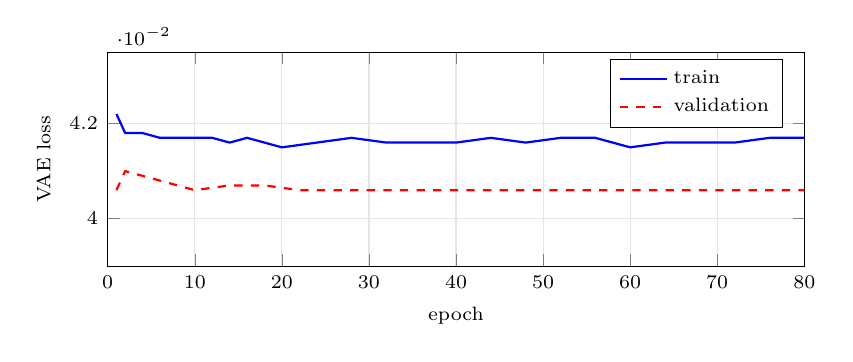
\begin{tikzpicture}
\begin{axis}[width=0.86\columnwidth,height=4.3cm,
  xlabel={epoch},ylabel={VAE loss},
  ymin=0.039,ymax=0.0435,xmin=0,xmax=80,
  legend pos=north east,legend cell align=left,
  grid=both,grid style={gray!20},tick label style={font=\scriptsize},
  label style={font=\scriptsize},legend style={font=\scriptsize}]
\addplot[thick,blue,mark=none] coordinates {(1,0.0422) (2,0.0418) (4,0.0418) (6,0.0417) (8,0.0417) (10,0.0417) (12,0.0417) (14,0.0416) (16,0.0417) (20,0.0415) (24,0.0416) (28,0.0417) (32,0.0416) (36,0.0416) (40,0.0416) (44,0.0417) (48,0.0416) (52,0.0417) (56,0.0417) (60,0.0415) (64,0.0416) (68,0.0416) (72,0.0416) (76,0.0417) (80,0.0417)};
\addplot[thick,red,dashed,mark=none] coordinates {(1,0.0406) (2,0.0410) (4,0.0409) (6,0.0408) (8,0.0407) (10,0.0406) (14,0.0407) (18,0.0407) (22,0.0406) (26,0.0406) (30,0.0406) (34,0.0406) (40,0.0406) (46,0.0406) (52,0.0406) (58,0.0406) (64,0.0406) (70,0.0406) (76,0.0406) (80,0.0406)};
\legend{train,validation}
\end{axis}
\end{tikzpicture}
\caption{\texttt{learned-vae} training and validation loss per epoch ($P_6$, $1560/312$
train/val graphs). Validation tracks training and stays slightly below it---no
overfitting; the fast plateau reflects the multimodal centroid target (model
selection uses the downstream validation ACL, not this loss).}
\label{fig:vaeloss}
\end{figure}

\subsection{The collapse, and a symmetry-invariant fix}
\label{sec:learn-collapse}

\paragraph{The audit.} The flat loss of Fig.~\ref{fig:vaeloss} is a genuine
\emph{posterior collapse}. Probing the trained model confirms it predicts the
\emph{same constant coordinate} for every vertex of every graph (per-graph prediction
spread $=0$), and its reconstruction MSE equals, to three digits, that of a predictor
that just outputs the global-mean centroid; the supervised \texttt{learned-gnn-seed}
collapses identically. What then produced the apparent $1.947$ ACL of
\texttt{learned-vae}? \emph{Only its best-of-$K$ wrapper.} Because the layout is
constant, the $K{=}8$ samples differ solely in their \texttt{minorminer} random seed,
so \texttt{learned-vae} \emph{is} best-of-$8$ cold \texttt{minorminer}. On a matched
sample it ties---indeed marginally loses to---plain best-of-$8$ \texttt{minorminer}
($2.097$ vs.\ $2.086$); its edge over \texttt{reweave-thorough} was simply $8$
restarts versus $4$. \textbf{We therefore retract the earlier reading that a learned
model beat Reweave-thorough}: it was an unequal-budget artifact on top of a
collapsed model.

\paragraph{Why it collapses, and the fix.}
\label{sec:learn-fix}
The target is ill-posed: regressing an \emph{absolute} hardware coordinate asks the
model for something the graph does not determine, because the embedding is free under
the fabric's translation/rotation/reflection symmetries. We remove that freedom with a
\textbf{Procrustes} (similarity-invariant) loss: per graph, align the predicted layout
to the target up to rotation, reflection, scale and translation (a closed-form,
differentiable Kabsch step) \emph{before} the MSE, so the loss sees only the
\emph{relative} structure---which the graph \emph{does} determine. This cures the
collapse (non-zero spread; adjacent vertices placed closer than non-adjacent), and the
resulting \texttt{learned-procrustes} layout is the method we evaluate below.

\subsection{Fair, equal-budget results}
\label{sec:learn-results}

The honest comparison gives every method the \emph{same} decode budget---single-shot
is one \texttt{minorminer} call, best-of-$8$ is eight---and asks whether the learned
layout helps (Table~\ref{tab:learn-quality}; held-out test set, $312$ instance-disjoint
graphs, clean $P_6$).

\begin{table}[t]
\caption{Fair, equal-budget held-out comparison on clean Pegasus $P_6$ ($312$ graphs,
all $100\%$ valid). Mean ACL, lower better; $p$ is a per-graph paired Wilcoxon test
vs.\ cold \texttt{minorminer} at the \emph{same} budget.}
\label{tab:learn-quality}
\small
\begin{tabular}{lrr}
\toprule
method & mean ACL & $p$ vs.\ cold MM\\
\midrule
single cold \texttt{minorminer}        & 2.072 & ---\\
\texttt{learned-procrustes}            & 2.056 & $0.047$\\
\quad + decode-aware RL                & 2.040 & $4{\times}10^{-4}$\\
\midrule
best-of-$8$ cold \texttt{minorminer}   & 1.943 & ---\\
\texttt{learned-procrustes-k8}         & 1.925 & ${<}10^{-3}$\\
\quad + decode-aware RL                & 1.927 & $1{\times}10^{-4}$\\
\bottomrule
\end{tabular}
\end{table}

So the symmetry-fixed layout \textbf{beats \texttt{minorminer} at equal budget on both
ends}---$-0.8\%$ single-shot and $-0.9\%$ in best-of-$8$, each statistically
significant. The magnitude is small: a fixed $2$-D layout maps only loosely onto
Pegasus hop-distance, and \texttt{minorminer}'s cold search with restarts is already
strong. The other families confirm the picture---the collapsed \texttt{learned-gnn-seed},
the non-neural \texttt{learned-retrieve} embeddings-cache~\cite{brahm2021caching}, and the label-free
\texttt{learned-obj} (which trains a layout to minimize an edge-stretch objective and
does \emph{not} collapse) all land within noise of \texttt{minorminer}.

\paragraph{Decode-aware RL does not break the ceiling.} To try to push past the
supervised layout, we fine-tuned it with REINFORCE \emph{through} the decoder: the
policy is a Gaussian around the predicted layout, the reward is the per-graph-baselined
negative decoded ACL, with a Procrustes anchor for stability. It nudges single-shot ACL
to $2.040$ ($-1.5\%$ vs.\ \texttt{minorminer}, $p{=}4{\times}10^{-4}$; line ``$+$RL'' in
Table~\ref{tab:learn-quality}) but does \emph{not} significantly beat the supervised
layout ($p{=}0.06$) and is unstable---the validation gain drifts \emph{down} with more
epochs across two independent runs. Optimizing the true objective directly
\emph{confirms} the ceiling rather than lifting it: the limit is the placement action
space, not the training signal.

\paragraph{Verdict, and what is honestly true.} Learning helps here, but \emph{modestly
and only after the symmetry fix}. The contribution is the diagnosis (the naive
supervised target is ill-posed and collapses) and the cure (a Procrustes-invariant
objective), which turns a constant-predicting model into one that beats
\texttt{minorminer} by ${\sim}1\%$ at equal budget. It does not beat best-of-$K$
\texttt{minorminer} by much, and decode-aware RL does not exceed it---so a strong
heuristic with restarts remains hard to beat with learned \emph{placement}. The
premise of the deep-learning embedding patent~\cite{hyde2025dlembedding} is thus
partly borne out: a learned model yields a small, real
improvement, but it is no substitute for a good heuristic. Validity is never at risk:
the seed$\rightarrow$MM decoder always falls back to a cold \texttt{minorminer} call, so
every learned method is $100\%$-valid in the same sense \texttt{minorminer} is---it
inherits \texttt{minorminer}'s completeness and the learned layout changes only the
\emph{quality} of the result, never its validity.

%% ========================================================================
\section{Guiding the Search: Vertex Order and Rip-Up}
\label{sec:searchguide}

Reweave improves the embedding \texttt{minorminer} produces, and \S\ref{sec:learning}
tried to \emph{learn} a better one; this section attacks a third, orthogonal lever---the
\emph{order} in which \texttt{minorminer} searches. Any \texttt{minorminer}-style
embedder exposes two such order levers: the \textbf{vertex order} in which chains are
built and rebuilt, and the \textbf{rip-up policy} that chooses which chain to tear out
and reroute next. \texttt{minorminer}'s own authors named initial placement and vertex
order as the key open problem, and much of its run-to-run variance is order-driven---yet,
to our knowledge, search-order heuristics for minor embedding are unstudied. We test both levers, deterministically and
with a learned model, in three vehicles: Reweave, a small fork of
\texttt{minorminer} that exposes its variable order, and \texttt{minorminer}'s own
\texttt{quickpass} greedy primitive.

\paragraph{Opening \texttt{minorminer}'s variable order.}
Stock \texttt{find\_embedding} runs its full heuristic---tear-and-replace plus
\texttt{tries} restarts---under an \emph{internal randomized} order, and offers no
way to supply one (only the much weaker \texttt{quickpass} primitive takes a custom
order). We forked \texttt{minorminer}~0.2.22 with a ${\sim}90$-line patch that adds
a \texttt{var\_order} parameter threaded into every pass of the full search: an
\texttt{optional\_parameters} field, an early return in the variable-order routine
(guarded so the per-connected-component subproblems fall back to the default), and
the Cython binding plumbing. \emph{Without} \texttt{var\_order} the fork is
byte-identical to stock \texttt{minorminer} (parity-tested across seeds, once the
public wrapper's default \texttt{tries}{=}$10$ is matched); the patch and a
one-command build ship in the artifact (\texttt{scripts/build\_mm\_fork.sh}). The
guided search is exposed as \texttt{mmfork} (no order---the stock-MM control) and
\texttt{mmfork-}$\langle\textit{order}\rangle$.

\paragraph{Rip-up selection is a dead lever.}
We added five rip-up \emph{selection} policies to Reweave's dirty-set improver
(longest-first, boundary-churn, contention, inflation, and a contrarian
shortest-first), changing only \emph{which} chain is attacked next while holding
the move operator and accept rule byte-for-byte. On the dense grid (six LNS-active
cells, three seeds) all five land within $0.004$ ACL of the default---even
shortest-first. The improver converges to essentially the same local optimum
regardless of rip-up order, so the FPGA ``which-net-to-rip'' idea has no quality
headroom here and we did not pursue a learned rip-up policy. (That
\texttt{reweave-ripup-longest} reproduces \texttt{reweave} exactly also validates
the refactored loop.)

\paragraph{Vertex order is a real lever.}
On the forked full search a bandwidth/locality order---reverse Cuthill--McKee---
lowers mean ACL, and because \texttt{minorminer}'s variance on these feasible
instances is order-driven it also cuts run-to-run variance by ${\sim}25\%$
(Table~\ref{tab:mmfork}). Order quality is vehicle- and instance-dependent
(\texttt{minfill} wins on the weak \texttt{quickpass} primitive, \texttt{cuthill}
on the full search; \texttt{degeneracy} and \texttt{community} can hurt), which is
exactly why a per-instance \textbf{portfolio}---run the five good orders, keep the
best valid embedding---is so effective: \texttt{mmfork-portfolio} reaches $-5.3\%$
ACL vs.\ \texttt{minorminer} and $-3.1\%$ vs.\ \texttt{reweave} at roughly
\emph{half} \texttt{minorminer}'s variance, the strongest single quality result in
this paper, at ${\sim}6\times$ the wall-clock since it runs every order.

\begin{table}[t]
\caption{Order-guided \texttt{minorminer} on the full search (standard grid: ER
sources over a size/density/topology mix, $7$ cells, $3$ seeds; mean ACL, std over
cell means in parentheses; lower is better). \texttt{mmfork} (no order) reproduces
\texttt{minorminer} exactly. A fixed Cuthill--McKee order and especially the
per-instance portfolio cut both ACL and variance. The last column is wall-clock
relative to \texttt{minorminer} (Table~\ref{tab:fgtime}): a single fixed order is
free, the portfolio runs every order.}
\label{tab:mmfork}
\small
\begin{tabular}{lcccc}
\toprule
algorithm & ACL (std) & vs.\ MM & vs.\ Reweave & $t/$MM \\
\midrule
\texttt{minorminer} $\equiv$ \texttt{mmfork} & 3.641 (0.115) & --- & $+2.4\%$ & $1.0\times$ \\
\texttt{mmfork-cuthill}    & 3.592 (0.105) & $-1.6\%$ & $+0.8\%$ & $1.0\times$ \\
\texttt{reweave}           & 3.553 (0.102) & $-2.3\%$ & --- & $1.7\times$ \\
\textbf{\texttt{mmfork-portfolio}} & \textbf{3.456} (\textbf{0.059}) & $\mathbf{-5.3\%}$ & $\mathbf{-3.1\%}$ & $5.9\times$ \\
\bottomrule
\end{tabular}
\end{table}

\paragraph{The new embedders stack with Reweave.}
Reweave warm-starts from any registered base embedder and then improves it, so the
order-guided variants compose with it directly. The \emph{lowest} ACL we observe
comes from seeding Reweave with \texttt{mmfork-portfolio} (\texttt{reweave+mmfork} in
Table~\ref{tab:stack}): it stacks two independent gains---a better-ordered base
\emph{and} the negotiated destroy-repair improver---but inherits the portfolio's
${\sim}6\times$ cost as its base. The practical sweet spot is to seed from the single
Cuthill order instead: \texttt{reweave-mmfork-cuthill} reaches ${\sim}{-}5\%$ ACL
versus \texttt{minorminer}---matching the ${\sim}6\times$ portfolio and beating both
plain \texttt{reweave} ($-3.4\%$) and \texttt{mmfork-cuthill} ($-2.2\%$) on their
own---at only ${\sim}1.8\times$ \texttt{minorminer}, the cost of plain Reweave. The
levers are orthogonal: ordering improves the base, Reweave's improver improves
whatever base it is given (the same composition mechanism as the existing
\texttt{reweave-stacked} variant, which seeds from the multilevel placement).

\begin{table}[t]
\caption{The quality/speed spectrum of the order-guided embedders and their stacks
(ER into $P_6$, mean over four size/density cells $\times3$ seeds; $t/$MM is
wall-clock relative to \texttt{minorminer}, back-to-back). The cheap stack,
\textbf{\texttt{reweave-mmfork-cuthill}}, matches the ${\sim}6.5\times$ portfolio's
ACL at plain Reweave's cost; only the portfolio-seeded \texttt{reweave+mmfork} goes
lower, and it pays the portfolio's ${\sim}6\times$ as its base.}
\label{tab:stack}
\small
\begin{tabular}{lccc}
\toprule
method & ACL & vs.\ MM & $t/$MM \\
\midrule
\texttt{minorminer}                  & 5.233 & ---      & $1.0\times$ \\
\texttt{mmfork-cuthill}              & 5.117 & $-2.2\%$ & $1.0\times$ \\
\texttt{reweave}                     & 5.055 & $-3.4\%$ & $2.0\times$ \\
\textbf{\texttt{reweave-mmfork-cuthill}} & \textbf{4.960} & $\mathbf{-5.2\%}$ & $\mathbf{1.8\times}$ \\
\texttt{mmfork-portfolio}            & 4.949 & $-5.4\%$ & $6.5\times$\,/\,$1.7\times^{\dagger}$ \\
\texttt{reweave+mmfork} (portf.)     & \textbf{4.801} & $-8.3\%$ & $7.4\times$ \\
\bottomrule
\end{tabular}

{\footnotesize $^{\dagger}$\,\texttt{mmfork-portfolio-par}: the portfolio's
independent orders run on a fork process pool (${\sim}3.5\times$ speedup,
identical ACL).}
\end{table}

\paragraph{Timing.} Guiding the order is nearly free, so the single-order variants
are drop-ins on \emph{speed} as well as quality. The order is computed once in
$O(|V|{+}|E|)$ and the search is otherwise \texttt{minorminer}'s, so over the
standard grid \texttt{mmfork} is identical to \texttt{minorminer} ($1.0\times$) and
\texttt{mmfork-cuthill} averages $1.0\times$---a good order even converges
marginally faster, and it is faster than \texttt{minorminer-layout} ($1.3\times$).
The portfolio buys its quality and variance with a constant factor of time: it runs
the five orders plus the default, so serially \texttt{mmfork-portfolio} is
$5.9\times$ \texttt{minorminer}. Its orders are independent, however, so a
process-parallel variant (\texttt{mmfork-portfolio-par}) recovers ${\sim}3.5\times$
of that on a multi-core host---at \emph{identical} ACL---bringing a single embedding
back to ${\sim}1.7\times$. The $6.4\times$ of \texttt{reweave+mmfork}
(Table~\ref{tab:fgtime}) deserves a word, because it is \emph{not}
reweave\,($1.7\times$) plus mmfork\,($1.0\times$): it is Reweave seeded from the
\emph{portfolio} base, so it pays the portfolio's ${\sim}6\times$. Seeding instead
from the single Cuthill order (\texttt{reweave-mmfork-cuthill}) gives nearly the same
ACL at ${\sim}1.8\times$, which is the configuration to use. Finally, reducing
\texttt{minorminer}'s restart count does \emph{not} speed the single-order variants:
under a fixed order the redundant restarts short-circuit, so \texttt{tries}$\in\{1,
\dots,10\}$ give identical ACL \emph{and} wall-clock (e.g.\ on a $P_{16}$,
$n{=}80$ instance, ACL ${\approx}8.14$ and ${\sim}15$\,s for \emph{every}
\texttt{tries})---the single fixed order is already as fast as the search gets. Table~\ref{tab:fgtime} gives per-cell seconds;
all algorithms run back-to-back on each instance so the ratios are robust to CPU
contention.

\begin{table}[t]
\caption{Wall-clock for the search-guidance algorithms (mean seconds per embedding;
all algorithms run back-to-back per (cell, seed) so ratios are contention-robust;
$30$\,s budget). Single-order \texttt{mmfork-cuthill} matches \texttt{minorminer}
(\texttt{mmfork} without an order is identical, omitted); the portfolio and the
stacked variant cost a ${\sim}6\times$ constant factor.
\texttt{mm}${=}$\texttt{minorminer}, \texttt{mm-l}${=}$\texttt{minorminer-layout},
\texttt{mf}${=}$\texttt{mmfork}.}
\label{tab:fgtime}
\small
\begin{tabular}{lrrrrr}
\toprule
cell & \texttt{mm} & \texttt{mm-l} & \texttt{mf-cuth} & \texttt{mf-portf} & \texttt{rw+mf} \\
\midrule
$n{=}20,d{=}0.5$         & 0.09 & 0.09 & 0.14 & 0.69 & 0.67 \\
$n{=}30,d{=}0.5$         & 0.53 & 0.37 & 0.36 & 2.43 & 2.51 \\
$n{=}30,d{=}0.7$         & 0.77 & 0.76 & 0.94 & 3.53 & 3.80 \\
$n{=}40,d{=}0.5$         & 1.01 & 0.86 & 0.72 & 5.41 & 5.76 \\
$n{=}40,d{=}0.7$         & 1.13 & 1.67 & 1.04 & 6.44 & 6.94 \\
$n{=}60,d{=}0.5$         & 0.95 & 2.00 & 1.25 & 7.49 & 8.73 \\
$n{=}30,d{=}0.5$ (broken)& 0.34 & 0.41 & 0.35 & 2.30 & 2.34 \\
$n{=}30,d{=}0.5$ ($Z_4$) & 0.27 & 0.35 & 0.23 & 1.65 & 1.75 \\
\midrule
mean $\times$\,\texttt{mm} & $1.0$ & $1.3$ & $1.0$ & $5.9$ & $6.4$ \\
\bottomrule
\end{tabular}
\end{table}

\paragraph{Drop-in safety: as reliable as \texttt{minorminer}.}
A natural worry is whether fixing one order across all restarts---removing the
order diversity \texttt{minorminer} relies on near the feasibility boundary---makes
the guided search \emph{fail} where stock \texttt{minorminer} would succeed, the
way constructive embedders such as ATOM fail outright on hard instances. We ensure
the new embedders are genuine drop-ins. \texttt{mmfork} is stock
\texttt{minorminer}; \texttt{mmfork-portfolio} always includes a stock-MM config;
and each single-order \texttt{mmfork-}$\langle\textit{order}\rangle$ falls back to
one stock-\texttt{minorminer} call if its ordered attempt fails---so success rate is
$\geq$ \texttt{minorminer} \emph{by construction}. Table~\ref{tab:success} confirms
this empirically and then some: forced into \texttt{minorminer}'s partial-success
regime by a short ($8$\,s) budget on dense cells, the fixed Cuthill--McKee order
\emph{matches or exceeds} stock \texttt{minorminer}'s success rate---dramatically so
on the hardest cell, $8/8$ versus $2/8$ (Table~\ref{tab:success}). A good order is
at least as reliable as a random one and, near the boundary, expands the
feasibility frontier as well as shortening chains; the fall-back (never even
triggered here) is a guarantee rather than a crutch. Crucially, every
\texttt{mmfork} output is a genuine \texttt{minorminer} embedding, so validity is
never at risk and these variants are $100\%$-valid in the same sense
\texttt{minorminer} is---unlike a constructive embedder, they cannot fail where
\texttt{minorminer} would not.

\begin{table}[t]
\caption{Drop-in reliability near \texttt{minorminer}'s feasibility boundary (ER
into $P_6$, $8$\,s budget, $8$ seeds; valid embeddings found). A fixed
Cuthill--McKee order is at least as reliable as stock \texttt{minorminer} and
markedly more so on the hardest cell; the stock-MM fall-back (not triggered here)
guarantees success $\geq$ \texttt{minorminer} regardless.}
\label{tab:success}
\small
\begin{tabular}{lccc}
\toprule
cell & \texttt{minorminer} & \texttt{mmfork-cuthill} (no fb) & \texttt{mmfork-cuthill} \\
\midrule
$n{=}63,d{=}0.5$ & 8/8 & 8/8 & 8/8 \\
$n{=}64,d{=}0.5$ & 7/8 & 8/8 & 8/8 \\
$n{=}65,d{=}0.5$ & 2/8 & \textbf{8/8} & \textbf{8/8} \\
\bottomrule
\end{tabular}
\end{table}

\paragraph{Learning does not beat the best fixed order.}
Finally we tested whether a model can pick or generate a per-instance order that
beats the fixed heuristics, applying the same ceiling-probe discipline as
\S\ref{sec:learning}: a cheap linear model first, escalating to a GNN only if it
shows headroom. On an instance-disjoint test set (47 graphs), an order
\emph{selector} (graph features $\rightarrow$ which fixed order to run) reaches
$-1.9\%$ ACL vs.\ \texttt{minorminer}---statistically a tie with simply always
using Cuthill--McKee ($-1.8\%$), and far from the per-instance oracle ($-4.6\%$);
a learned per-vertex \emph{score} (features $\rightarrow$ order, weights
hill-climbed with the forked search in the loop) gives $-0.2\%$, no better than the
heuristics, its weights collapsing to a degeneracy-like prior. Graph-level features
do not predict which order wins, so the cheap model amounts to ``use
Cuthill--McKee'' and a GNN on the cluster was not warranted---the same ceiling the
learned-placement study of \S\ref{sec:learning} hit. The real opportunity the
oracle exposes ($-4.6\%$) is a \emph{cheaper} portfolio, not a learned order.

\paragraph{Verdict.} Of the two search levers, rip-up selection is inert but vertex
order is real: a deterministic Cuthill--McKee order, or better a per-instance
portfolio, lowers \texttt{minorminer}'s ACL by up to $5\%$ and halves its variance,
composes with Reweave for the best result overall, and---unlike a learned or
constructive embedder---never sacrifices \texttt{minorminer}'s reliability. The full
study, including the cross-vehicle results and the negative rip-up and learning
findings, is in \texttt{docs/candidate-algorithms/search-guidance/}.

%% ========================================================================
\section{Scaling Behaviour on Advantage and Advantage2}
\label{sec:scaling}

The experiments so far target a small graph, Pegasus $P_6$ ($680$ qubits). To see
how the methods behave at the scale of \emph{real} hardware we repeat the
comparison on the actual D-Wave topologies---Advantage's Pegasus $P_{16}$
($5640$ qubits) and Advantage2's Zephyr $Z_{15}$ ($7440$ qubits), each with $5\%$
simulated dead qubits, a realistic working graph---and sweep the source size $n$
from small to large under two regimes: Erd\H{o}s--R\'enyi at fixed density
($d{=}0.3$) and $6$-regular at fixed degree (which stays sparse and so reaches much
larger $n$). The full grid runs on a $128$-core host; we report ACL, success, and
wall-clock versus $n$.

\paragraph{The relative cost of guidance shrinks with $n$.} The headline is the
time curve (Figure~\ref{fig:scaling}): the wall-clock multipliers of all the guided
methods \emph{fall} as the problem grows. On $Z_{15}$, \texttt{mmfork-cuthill} drops
from $1.3\times$ \texttt{minorminer} at $n{=}40$ to $0.6\times$ at $n{=}320$---i.e.\
it becomes \emph{faster} than stock \texttt{minorminer} at scale, because a good
fixed order reaches a valid embedding before \texttt{minorminer}'s randomized search
does; \texttt{reweave-mmfork-cuthill} falls from $1.7\times$ to $0.9\times$, and even
the six-search portfolio's multiplier nearly halves ($7.3\times{\to}4.4\times$).
$P_{16}$ is the same story ($\texttt{mmfork-cuthill}\,1.5\times{\to}1.0\times$, the
portfolio $8.2\times{\to}5.3\times$). So the fixed overhead of computing an order, or
of running several of them, amortizes against \texttt{minorminer}'s
super-linearly-growing search: a method that is slower at small $n$ is relatively
cheaper---sometimes free---at the large $n$ that real hardware makes reachable. The
single-order variants are therefore an unambiguous win at scale, and even the
portfolio's premium is far smaller on big problems than the ${\sim}6\times$ measured
on $P_6$.

\begin{figure}[t]
\centering
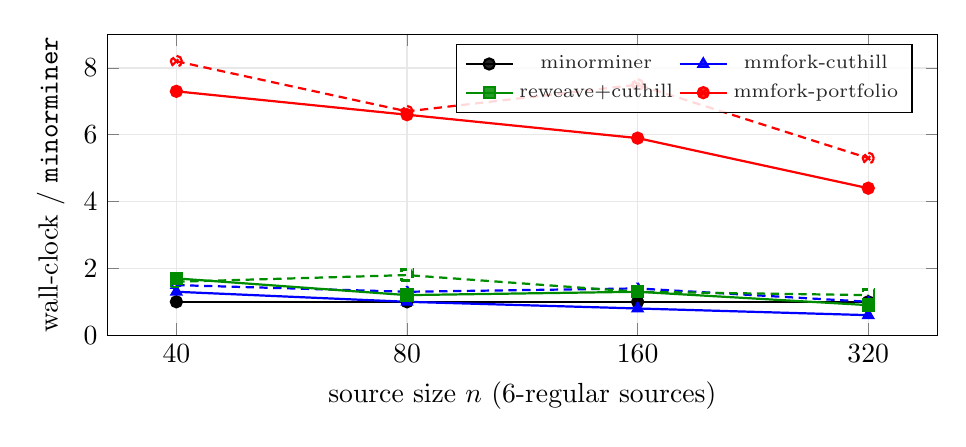
\begin{tikzpicture}
\begin{axis}[width=\linewidth, height=5.4cm, xmode=log, log basis x=2,
  xtick={40,80,160,320}, xticklabels={40,80,160,320},
  xlabel={source size $n$ ($6$-regular sources)},
  ylabel={wall-clock $/$ \texttt{minorminer}}, ymin=0, ymax=9,
  legend pos=north east, legend columns=2,
  legend style={font=\scriptsize, fill opacity=0.85},
  grid=both, grid style={gray!18}]
\addplot[black,thick,mark=*] coordinates {(40,1)(80,1)(160,1)(320,1)}; \addlegendentry{minorminer}
\addplot[blue,thick,mark=triangle*] coordinates {(40,1.3)(80,1.0)(160,0.8)(320,0.6)}; \addlegendentry{mmfork-cuthill}
\addplot[blue,thick,densely dashed,mark=triangle,forget plot] coordinates {(40,1.5)(80,1.3)(160,1.4)(320,1.0)};
\addplot[green!55!black,thick,mark=square*] coordinates {(40,1.7)(80,1.2)(160,1.3)(320,0.9)}; \addlegendentry{reweave+cuthill}
\addplot[green!55!black,thick,densely dashed,mark=square,forget plot] coordinates {(40,1.6)(80,1.8)(160,1.3)(320,1.2)};
\addplot[red,thick,mark=otimes*] coordinates {(40,7.3)(80,6.6)(160,5.9)(320,4.4)}; \addlegendentry{mmfork-portfolio}
\addplot[red,thick,densely dashed,mark=otimes,forget plot] coordinates {(40,8.2)(80,6.7)(160,7.5)(320,5.3)};
\end{axis}
\end{tikzpicture}
\caption{Wall-clock relative to \texttt{minorminer} ($=1$) versus source size $n$
($6$-regular sources; \textbf{solid} $=$ Advantage2 $Z_{15}$, \textbf{dashed} $=$
Advantage $P_{16}$; $5\%$ faults). Every guided method's multiplier \emph{shrinks}
with $n$: \texttt{mmfork-cuthill} and \texttt{reweave-mmfork-cuthill} fall
\emph{below} $1$ (faster than stock \texttt{minorminer}) on the largest $Z_{15}$
problems, and even the six-search portfolio's premium nearly halves. The fixed cost
of guidance amortizes against \texttt{minorminer}'s super-linearly-growing search.}
\label{fig:scaling}
\end{figure}

\paragraph{Quality stays competitive; the frontier is shared.} On ACL the portfolio
and \texttt{reweave-mmfork-cuthill} remain at or ahead of \texttt{minorminer} across
the swept sizes (Figure~\ref{fig:scalingacl})---by up to ${\sim}10\%$ at the densest
feasible cell---though with a single source instance per size the per-$n$ gains are
noisy and not monotone, so we do not claim the ACL advantage \emph{widens} with $n$,
only that it persists. The
\emph{feasibility} frontier is shared: every method succeeds together up to
$n{=}320$ ($6$-regular) and $n{=}120$ (ER $d{=}0.3$) on $P_{16}$ and then fails
together beyond---this is the hardware's capacity limit, not an algorithmic one, and
is distinct from the near-boundary success advantage of Table~\ref{tab:success}
(which concerns \texttt{minorminer}'s \emph{stochastic} limit at a fixed size, where
a good order does help). The practical takeaway: on real Advantage/Advantage2
hardware the order-guided variants keep \texttt{minorminer}'s reach and reliability
while their time premium vanishes with scale, making \texttt{mmfork-cuthill} (and,
for the best quality, \texttt{reweave-mmfork-cuthill}) the preferred drop-ins for
large problems.

\begin{figure}[t]
\centering
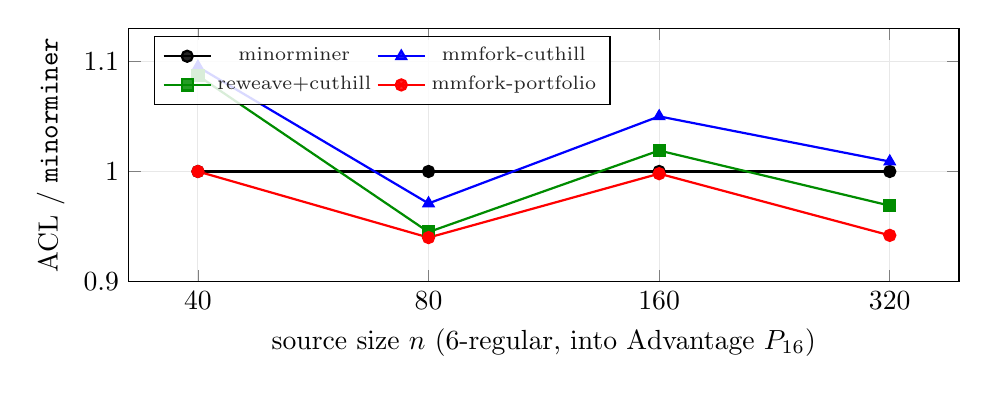
\begin{tikzpicture}
\begin{axis}[width=\linewidth, height=4.8cm, xmode=log, log basis x=2,
  xtick={40,80,160,320}, xticklabels={40,80,160,320},
  xlabel={source size $n$ ($6$-regular, into Advantage $P_{16}$)},
  ylabel={ACL $/$ \texttt{minorminer}}, ymin=0.9, ymax=1.13,
  legend pos=north west, legend columns=2,
  legend style={font=\scriptsize, fill opacity=0.85},
  grid=both, grid style={gray!18}]
\addplot[black,thick,mark=*] coordinates {(40,1)(80,1)(160,1)(320,1)}; \addlegendentry{minorminer}
\addplot[blue,thick,mark=triangle*] coordinates {(40,1.095)(80,0.971)(160,1.050)(320,1.009)}; \addlegendentry{mmfork-cuthill}
\addplot[green!55!black,thick,mark=square*] coordinates {(40,1.087)(80,0.945)(160,1.019)(320,0.969)}; \addlegendentry{reweave+cuthill}
\addplot[red,thick,mark=otimes*] coordinates {(40,1.0)(80,0.940)(160,0.998)(320,0.942)}; \addlegendentry{mmfork-portfolio}
\end{axis}
\end{tikzpicture}
\caption{ACL relative to \texttt{minorminer} ($=1$) versus $n$ ($6$-regular into
Advantage $P_{16}$). \texttt{mmfork-portfolio} and \texttt{reweave-mmfork-cuthill}
sit at or below $1$ (at-or-better-than \texttt{minorminer}) across scales; with one
source instance per size the curves are noisy, so the quality advantage
\emph{persists} rather than clearly widening with $n$.}
\label{fig:scalingacl}
\end{figure}

%% ========================================================================
\section{Solution Quality on a Simulator}
\label{sec:solquality}

Every result so far optimizes \emph{average chain length}: we treat ACL (and its
variance) as a proxy for the quantity a practitioner cares about---the quality of
the solutions a quantum annealer returns. That proxy is standard, and the
state-of-the-art evaluation we follow adopts it because ACL is the structural metric
that correlates most strongly with annealing solution error~\cite{gomez2025eval}.
But the paper never tests the link directly. This section does, on a simulator: we
put random Ising problems on the source graphs, embed each with every method, sample
the embedded problem, and ask whether shorter-ACL embeddings actually yield better
solutions.

\paragraph{Protocol.} For each source graph we draw random Ising problems with
$h_i,J_{ij}\in\{-1,+1\}$ and compute the exact ground-state energy by brute force,
which bounds the sources to $n\le 18$. We embed every problem with all six methods
(two embedding seeds each) into clean and broken Pegasus~$P_3$---small enough that
the dense sources need real, breakable chains, so chain length matters---and build
the embedded Ising with the reference \texttt{dwave.embedding} construction
(ferromagnetic intra-chain couplers of strength $c$, swept as a multiple of
$\max|J|$). We sample each embedded problem with classical simulated
annealing~\cite{kirkpatrick1983sa,isakov2015sa} ($500$ reads, the optimized
\texttt{dwave.samplers} implementation), majority-vote unembed, and score against the
exact ground state. As a semiclassical quantum-annealing cross-check we repeat with
\emph{spin-vector Monte Carlo} (SVMC)~\cite{shin2014svmc}, in which each qubit is an
$O(2)$ rotor annealed under a transverse-field schedule. We report the
ground-state probability $P(\mathrm{GS})$, the residual-energy ratio
$(\langle E\rangle-E_0)/|E_0|$, and the chain-break fraction, over $114$ problems and
$2{,}736$ (problem, embedding) pairs.

\paragraph{Shorter chains give better solutions.} Across the whole cloud of
(problem, embedding) pairs, ACL is strongly and significantly anti-correlated with
solution quality: at the reference chain strength the Spearman correlation between ACL
and $P(\mathrm{GS})$ is $\rho=-0.63$ ($p\approx10^{-296}$), between ACL and residual
energy $\rho=+0.63$, and between ACL and chain breaks $\rho=+0.80$
(Figure~\ref{fig:quality}). The mechanism is direct---longer chains break more often
under a fixed coupler budget, and broken chains corrupt the majority vote. The link
is not an artifact of one chain-strength choice: taking each embedding's \emph{best}
strength over the sweep, ACL still predicts $P(\mathrm{GS})$ at $\rho=-0.53$
($p\approx10^{-197}$). Figure~\ref{fig:chainstrength} shows why: short chains are
already near-optimal at weak coupling, whereas long chains need a stronger
ferromagnet to hold together---and even fully compensated they top out lower, because
the coupler budget spent holding a long chain rigid is budget taken from the logical
problem.

\begin{figure}[t]
\centering
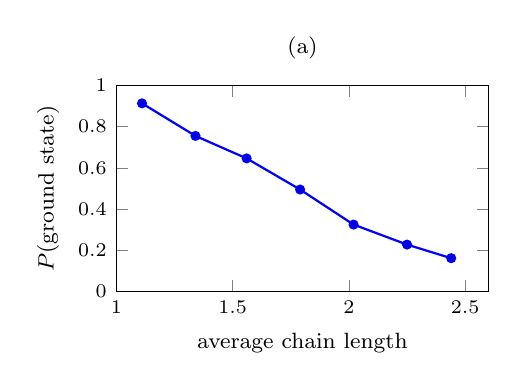
\begin{tikzpicture}
\begin{axis}[width=0.52\columnwidth, height=4.2cm,
  xlabel={average chain length}, ylabel={$P(\mathrm{ground\ state})$},
  ymin=0, ymax=1, xmin=1, xmax=2.6, title={(a)}, title style={font=\footnotesize},
  tick label style={font=\scriptsize}, label style={font=\footnotesize}]
\addplot+[thick,mark=*,mark size=1.4pt] coordinates
 {(1.11,0.913)(1.34,0.755)(1.56,0.646)(1.79,0.495)(2.02,0.325)(2.25,0.228)(2.44,0.162)};
\end{axis}
\end{tikzpicture}\hfill
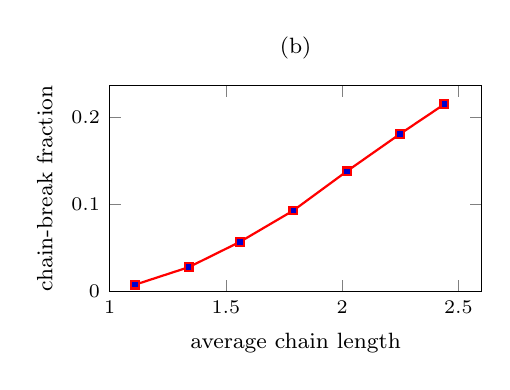
\begin{tikzpicture}
\begin{axis}[width=0.52\columnwidth, height=4.2cm,
  xlabel={average chain length}, ylabel={chain-break fraction},
  ymin=0, xmin=1, xmax=2.6, title={(b)}, title style={font=\footnotesize},
  tick label style={font=\scriptsize}, label style={font=\footnotesize}]
\addplot+[thick,mark=square*,mark size=1.4pt,red] coordinates
 {(1.11,0.008)(1.34,0.028)(1.56,0.057)(1.79,0.093)(2.02,0.138)(2.25,0.181)(2.44,0.215)};
\end{axis}
\end{tikzpicture}
\caption{Solution quality versus chain length across all $2{,}736$ (problem,
embedding) pairs (binned mean, reference chain strength). (a) the ground-state
probability falls monotonically with ACL ($\rho=-0.63$, $p\approx10^{-296}$); (b) the
chain-break fraction rises with ACL ($\rho=+0.80$)---the mechanism. Lower ACL is
better on both axes.}
\label{fig:quality}
\end{figure}

\begin{figure}[t]
\centering
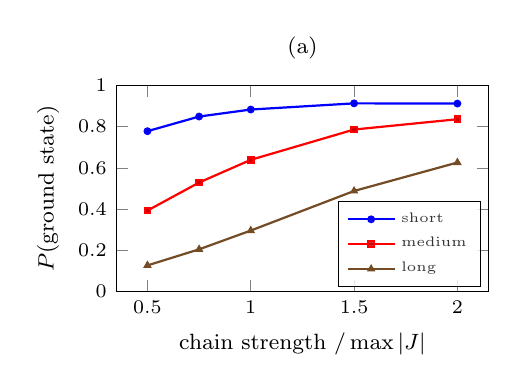
\begin{tikzpicture}
\begin{axis}[width=0.52\columnwidth, height=4.2cm,
  xlabel={chain strength $/\max|J|$}, ylabel={$P(\mathrm{ground\ state})$},
  ymin=0, ymax=1, title={(a)}, title style={font=\footnotesize},
  legend style={font=\tiny, at={(0.98,0.02)}, anchor=south east, fill opacity=0.8},
  legend cell align=left, tick label style={font=\scriptsize}, label style={font=\footnotesize}]
\addplot+[thick,mark=*,mark size=1pt] coordinates {(0.5,0.778)(0.75,0.849)(1.0,0.883)(1.5,0.913)(2.0,0.912)}; \addlegendentry{short}
\addplot+[thick,mark=square*,mark size=1pt] coordinates {(0.5,0.393)(0.75,0.529)(1.0,0.639)(1.5,0.786)(2.0,0.836)}; \addlegendentry{medium}
\addplot+[thick,mark=triangle*,mark size=1pt] coordinates {(0.5,0.127)(0.75,0.205)(1.0,0.296)(1.5,0.488)(2.0,0.626)}; \addlegendentry{long}
\end{axis}
\end{tikzpicture}\hfill
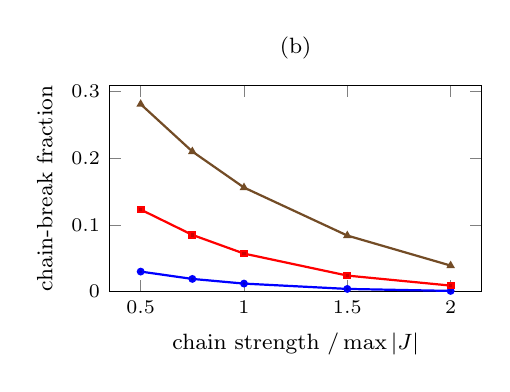
\begin{tikzpicture}
\begin{axis}[width=0.52\columnwidth, height=4.2cm,
  xlabel={chain strength $/\max|J|$}, ylabel={chain-break fraction},
  ymin=0, title={(b)}, title style={font=\footnotesize},
  tick label style={font=\scriptsize}, label style={font=\footnotesize}]
\addplot+[thick,mark=*,mark size=1pt] coordinates {(0.5,0.030)(0.75,0.019)(1.0,0.012)(1.5,0.004)(2.0,0.001)};
\addplot+[thick,mark=square*,mark size=1pt] coordinates {(0.5,0.123)(0.75,0.085)(1.0,0.057)(1.5,0.024)(2.0,0.009)};
\addplot+[thick,mark=triangle*,mark size=1pt] coordinates {(0.5,0.281)(0.75,0.210)(1.0,0.156)(1.5,0.084)(2.0,0.039)};
\end{axis}
\end{tikzpicture}
\caption{The chain-strength sweep, by ACL tertile (short $\le1.36$, medium, long
$\ge1.78$). (a) longer chains need a stronger ferromagnet and still cap at a lower
$P(\mathrm{GS})$; (b) at every chain strength the break fraction grows with chain
length. Spending coupler budget to hold long chains rigid is budget taken from the
logical problem---the cost that ACL measures.}
\label{fig:chainstrength}
\end{figure}

\paragraph{The shorter-ACL methods win on quality.} Ordered by mean
$P(\mathrm{GS})$, the methods rank exactly as their ACL predicts
(Table~\ref{tab:solquality}): \texttt{mmfork-portfolio} and \texttt{reweave-thorough},
the two lowest-ACL methods, give the highest ground-state probability, and
\texttt{mmfork-portfolio} beats \texttt{minorminer} on solution quality by a paired
Wilcoxon test across problems ($p=2\times10^{-4}$, medium effect). The per-method
\emph{gaps} are modest here because the brute-force ceiling forces small sources where
all methods produce short chains (ACL ${\approx}1.5$--$1.7$); the cloud-level
correlation, spanning the full ACL range, is the primary evidence and is overwhelming.
Simulated annealing and SVMC agree closely---they rank the six methods identically
(method-mean Spearman $\rho=0.94$; per-embedding $\rho=0.95$)---so the ordering is not
an artifact of one sampler.

\begin{table}[t]
\caption{Solution quality by method (mean over the $114$ problems, reference chain
strength, clean and broken $P_3$). Lower ACL tracks higher ground-state probability
under both samplers, lower residual energy, and fewer chain breaks.
$^{***}$\,$p<10^{-3}$, paired Wilcoxon vs.\ \texttt{minorminer}.}
\label{tab:solquality}
\small
\centering
\begin{tabular}{lccccc}
\toprule
method & ACL & $P_{\mathrm{SA}}(\mathrm{GS})$ & $P_{\mathrm{SVMC}}(\mathrm{GS})$ & resid. & break \\
\midrule
\texttt{minorminer} & 1.65 & 0.594 & 0.572 & 0.072 & 0.078 \\
\texttt{mm-layout} & 1.66 & 0.585 & 0.573 & 0.076 & 0.082 \\
\texttt{reweave} & 1.65 & 0.596 & 0.574 & 0.072 & 0.078 \\
\texttt{reweave-thorough} & 1.55 & 0.616 & 0.602 & 0.071 & 0.072 \\
\texttt{mmfork-cuthill} & 1.63 & 0.598 & 0.585 & 0.068 & 0.072 \\
\texttt{mmfork-portfolio} & 1.53 & 0.649$^{***}$ & 0.627 & 0.064 & 0.066 \\
\bottomrule
\end{tabular}

\end{table}

\paragraph{What this does and does not show.} Classical SA and semiclassical SVMC
exercise the pathway by which chain length degrades solutions on real hardware---chain
breaks and the dynamic-range tax of holding long chains together---which is the
dominant ACL-to-quality mechanism. They do not model coherent multi-qubit tunneling,
and a faithful open-system simulation of quantum annealing is infeasible at the
hundreds of physical qubits these embeddings occupy. The claim we support is therefore
the one the optimization rests on: \emph{at fixed problem and sampler, shorter and more
uniform chains yield measurably better solutions}, so the ACL reductions of the
preceding sections are reductions in something that matters.

%% ========================================================================
\section{Statistical Robustness Across Instances}
\label{sec:rigor}

The per-cell tables above follow the state-of-the-art protocol and isolate run-to-run
variance on \emph{one fixed graph instance} per cell---deliberately, because
single-instance seed spread is \texttt{minorminer}'s documented failure mode. It
leaves one question open: are the gains and the variance reduction properties of those
particular instances? To settle it we re-ran the entire grid with $K=15$ independent
graph instances per cell ($35$ cell--target combinations $\times\,15$ instances
$\times\,3$ seeds $=1{,}575$ embeddings per method), and analyze the $525$
per-(cell, target, instance) units with bootstrap confidence intervals and
Holm--Bonferroni-corrected paired Wilcoxon tests, separating graph-draw variance from
algorithm-seed variance.

The headline claims survive intact (Table~\ref{tab:instances}). \emph{Never-regress}
holds at the instance level: across all $525$ units, every Reweave configuration that
warm-starts from \texttt{minorminer} has mean ACL $\le$ \texttt{minorminer}'s, with a
maximum observed regression of $0.000$. The ACL reductions hold with tight
intervals---\texttt{reweave-thorough} $-5.4\%$ ($95\%$ CI $[-5.6,-5.1]$) and
\texttt{mmfork-portfolio} $-5.5\%$ $[-5.8,-5.3]$, both at $p<10^{-84}$ with large
effect size, and the cheap \texttt{reweave-mmfork-cuthill} stack $-1.7\%$
$[-2.0,-1.4]$. The \emph{variance} advantage---Reweave's central claim---is confirmed
once instance and seed variance are separated: \texttt{reweave-thorough} and
\texttt{mmfork-portfolio} cut the within-instance (seed) ACL standard deviation to
$0.54\times$ and $0.53\times$ \texttt{minorminer}'s, while their between-instance
standard deviation ($0.087$, $0.090$) is likewise below \texttt{minorminer}'s
($0.113$). The one variant that does \emph{not} survive scrutiny is
\texttt{reweave-stacked}: pooled over the grid it is $+2.6\%$ \emph{worse} than
\texttt{minorminer} and not significant, because its multilevel base inflates ACL on
small, sparse instances even as it helps on large dense ones (\S\ref{sec:optimizations})
---which is why we already report it as an optional variant rather than a default. The
multi-instance design turns that caveat from a hedge into a measurement.

\begin{table}[t]
\caption{The headline claims under $K=15$ instances per cell (pooled over all cells and
targets; $525$ paired per-(cell, target, instance) units). $\Delta$ACL is the mean
per-instance change vs.\ \texttt{minorminer} with a bootstrap $95\%$ CI; ``seed std''
is the within-instance ACL standard deviation and its ratio to \texttt{minorminer}'s;
$p$ is Holm-corrected paired Wilcoxon. $^{***}$\,significantly \emph{better} than
\texttt{minorminer} ($p<10^{-3}$); $^{\dagger}$\,significantly worse.}
\label{tab:instances}
\small
\centering
\begin{tabular}{lcccc}
\toprule
method & $\Delta$ACL vs.\ MM & 95\% CI & seed std (ratio) & paired $p$ \\
\midrule
\texttt{reweave-base} & $-0.8\%$$^{***}$ & $[-0.9,-0.7]$ & $0.122\,(0.93\times)$ & $9e{-}53$ \\
\texttt{reweave} & $-1.2\%$$^{***}$ & $[-1.4,-1.1]$ & $0.117\,(0.89\times)$ & $2e{-}54$ \\
\texttt{reweave-thorough} & $-5.4\%$$^{***}$ & $[-5.6,-5.1]$ & $0.071\,(0.54\times)$ & $1e{-}84$ \\
\texttt{mmfork-cuthill} & $-0.6\%$$^{***}$ & $[-0.9,-0.2]$ & $0.134\,(1.02\times)$ & $2e{-}4$ \\
\texttt{mmfork-portfolio} & $-5.5\%$$^{***}$ & $[-5.8,-5.3]$ & $0.070\,(0.53\times)$ & $2e{-}85$ \\
\texttt{reweave+cuthill} & $-1.7\%$$^{***}$ & $[-2.0,-1.4]$ & $0.119\,(0.91\times)$ & $8e{-}22$ \\
\texttt{reweave-stacked} & $+2.6\%$ & $[+1.7,+3.7]$ & $0.207\,(1.57\times)$ & $8e{-}1$ \\
\texttt{mm-layout} & $+0.7\%$$^{\dagger}$ & $[+0.4,+1.1]$ & $0.137\,(1.04\times)$ & $3e{-}2$ \\
\bottomrule
\end{tabular}

\end{table}

%% ========================================================================
\section{Limitations and Future Work}
\label{sec:limitations}

Reweave's wall-clock is at least \texttt{minorminer}'s \emph{by construction}:
it runs \texttt{minorminer} as its base and then improves the result, so it cannot
be faster than the baseline it builds on. The optimizations of
\S\ref{sec:optimizations} hold the improver's overhead to ${\sim}1.3\times$ via
bounded-region routing. Because \texttt{minorminer} is compiled C++ while our
improver is pure Python, we tested whether compiling the routing inner loop closes
the remaining gap, and found that it does not: a numba-compiled node-weighted
Dijkstra is several times faster than the pure-Python kernel on a full-graph search
in isolation, but inside the optimized router it yields no net speedup---bounded
routing has already shrunk each search to a small neighbourhood where the compiled
kernel's per-node advantage is cancelled by its call overhead, and replacing
bounded routing with a full-graph compiled search is ${\sim}24\%$ \emph{slower}.
Profiling further attributes $70$--$84\%$ of optimized-\texttt{reweave} runtime
to the compiled-C++ \texttt{minorminer} base call itself, which no Python-side or
C++ rewrite of our routing can touch. The ${\sim}1.3\times$ overhead therefore
reflects the genuine extra work of the improvement pass rather than interpreter
overhead, and the comparison against compiled \texttt{minorminer} is a fair one.
Reducing it further would mean doing \emph{less} improver work (fewer rounds, at a
quality cost) or finding a cheaper base than \texttt{minorminer}, rather than
compiling the existing inner loop; parallelized restarts would still cut the
thorough configuration's wall-clock. The standalone cold start
remains uncompetitive precisely because of the initial-placement problem; pairing
Reweave with a stronger global placement---e.g.\ a semi-relaxed
Gromov--Wasserstein assignment~\cite{vincentcuaz2022srgw}---is the natural next
step. The destroy-repair neighbourhood here is a single-chain shortcut;
a larger neighbourhood repaired exactly with a constraint solver
\cite{bernal2020ip} is a promising route to deeper ACL reductions. The
solution-quality validation of \S\ref{sec:solquality} is classical and semiclassical
by necessity: it exercises the chain-break and dynamic-range pathway that dominates
the ACL-to-quality link, but a faithful open-system quantum-annealing simulation at
the embedded sizes here remains out of reach, so direct confirmation on quantum
hardware is the natural next step.

%% ========================================================================
\section{Conclusion}
\label{sec:conclusion}

Minor-embedding chain construction is multi-net routing, and the routing
community has spent decades on exactly the two operations \texttt{minorminer}
performs weakly: building a net (Steiner tree) and resolving contention
(congestion). Importing a real Steiner inner step and negotiated congestion, run
as a warm-started anytime improver, yields Reweave---a drop-in method that never
regresses below \texttt{minorminer} and, in its thorough configuration, reduces
average chain length and---in nearly every cell---its run-to-run variance on
D-Wave Pegasus and Zephyr. A structured optimization pass (bounded routing,
dirty-set scheduling, spur-pruning) then makes the production algorithm
${\sim}3\times$ faster at equal-or-better quality, within ${\sim}1.3\times$
compiled \texttt{minorminer}'s wall-clock, so the gains come at little time cost.

The same diagnosis exposes a second, lighter lever. Much of
\texttt{minorminer}'s variance is \emph{order}-driven, so we open its vertex order
with a small fork: a bandwidth-reducing order, or a per-instance portfolio of
orders, lowers its ACL by up to ${\sim}5\%$ and roughly halves its variance,
composes with Reweave, and---unlike a learned or constructive embedder---never
sacrifices its reliability. On the actual Advantage and Advantage2 hardware graphs
this guidance is essentially free: its wall-clock premium vanishes as problems
grow. What does \emph{not} pay off is learning the placement: the naive supervised
model is ill-posed and collapses, a symmetry-invariant objective repairs it but
beats \texttt{minorminer} by only a small (if significant) ${\sim}1\%$, and
decode-aware reinforcement learning does not exceed it---so a strong heuristic with
restarts remains hard to beat with learned placement, and we report the failure
mode as carefully as the fix. Finally, we close the loop on the objective itself: a
simulator study over thousands of embedded Ising instances confirms that shorter,
more uniform chains yield significantly better annealing solutions---validating ACL
as more than a structural convenience---and a $K{=}15$-instance redesign with
confidence intervals and paired significance tests puts the headline gains and the
variance reduction on firm statistical footing, while honestly flagging the one
variant that does not survive it. The algorithmic primitives throughout are
classical; the contribution is their synthesis, application, and honest empirical
validation for minor embedding.

\appendix
\section{Complete per-cell results}
\label{app:full}

Table~\ref{tab:full} gives the average chain length, mean and standard deviation
over the five seeds, for every (source, target, algorithm) in the sweep---the
single source of truth for the aggregate statistics in \S\ref{sec:results}. Every
cell reaches $100\%$ success. Source families are ER (Erd\H{o}s--R\'enyi), reg
($d$-regular), and BA (Barab\'asi--Albert); the $d$-regular and BA sources are
run on clean Pegasus only. \texttt{reweave-thorough} attains the lowest ACL in
all $35$ cells, and \texttt{reweave} never exceeds \texttt{minorminer}.

\begin{table}[h]
\caption{Average chain length, mean\,(std) over $5$ seeds, for all $35$
instance--topology cells. Columns: \texttt{minorminer}, \texttt{minorminer-layout},
\texttt{reweave}, \texttt{reweave-thorough}.}
\label{tab:full}
\footnotesize
\setlength{\tabcolsep}{3.5pt}
\begin{tabular}{lcccc}
\toprule
cell & \texttt{mm} & \texttt{mm-lay} & \texttt{pathf} & \texttt{rw-thor} \\
\midrule
\multicolumn{5}{l}{\emph{Pegasus $P_6$ (clean)}}\\
\midrule
ER $n{=}20,d{=}0.3$ & 1.79\,(0.09) & 1.76\,(0.05) & 1.79\,(0.09) & 1.65\,(0.03) \\
ER $n{=}20,d{=}0.5$ & 2.28\,(0.12) & 2.34\,(0.06) & 2.25\,(0.07) & 2.19\,(0.04) \\
ER $n{=}20,d{=}0.7$ & 2.59\,(0.08) & 2.55\,(0.09) & 2.57\,(0.09) & 2.51\,(0.07) \\
ER $n{=}30,d{=}0.3$ & 2.70\,(0.11) & 2.75\,(0.15) & 2.69\,(0.10) & 2.59\,(0.03) \\
ER $n{=}30,d{=}0.5$ & 3.30\,(0.16) & 3.43\,(0.10) & 3.25\,(0.15) & 3.19\,(0.10) \\
ER $n{=}30,d{=}0.7$ & 3.83\,(0.22) & 3.80\,(0.17) & 3.79\,(0.23) & 3.65\,(0.06) \\
ER $n{=}40,d{=}0.3$ & 3.56\,(0.05) & 3.62\,(0.14) & 3.52\,(0.06) & 3.41\,(0.06) \\
ER $n{=}40,d{=}0.5$ & 4.57\,(0.10) & 4.72\,(0.13) & 4.49\,(0.14) & 4.38\,(0.08) \\
ER $n{=}40,d{=}0.7$ & 5.15\,(0.06) & 5.23\,(0.17) & 5.07\,(0.04) & 4.97\,(0.04) \\
reg $n{=}30,k{=}4$ & 1.37\,(0.06) & 1.41\,(0.11) & 1.37\,(0.06) & 1.31\,(0.03) \\
reg $n{=}30,k{=}6$ & 1.92\,(0.11) & 1.94\,(0.04) & 1.92\,(0.11) & 1.86\,(0.07) \\
reg $n{=}40,k{=}4$ & 1.51\,(0.12) & 1.48\,(0.06) & 1.51\,(0.11) & 1.35\,(0.04) \\
reg $n{=}40,k{=}6$ & 2.10\,(0.13) & 2.13\,(0.23) & 2.09\,(0.12) & 1.95\,(0.03) \\
BA $n{=}30,m{=}3$ & 1.56\,(0.11) & 1.51\,(0.07) & 1.56\,(0.11) & 1.50\,(0.06) \\
BA $n{=}30,m{=}5$ & 2.22\,(0.09) & 2.25\,(0.12) & 2.20\,(0.09) & 2.09\,(0.07) \\
BA $n{=}40,m{=}3$ & 1.80\,(0.06) & 1.73\,(0.08) & 1.79\,(0.06) & 1.71\,(0.09) \\
BA $n{=}40,m{=}5$ & 2.56\,(0.10) & 2.63\,(0.13) & 2.50\,(0.08) & 2.44\,(0.03) \\
\midrule
\multicolumn{5}{l}{\emph{broken Pegasus $P_6$ ($5\%$ faults)}}\\
\midrule
ER $n{=}20,d{=}0.3$ & 1.85\,(0.12) & 1.90\,(0.15) & 1.84\,(0.12) & 1.70\,(0.03) \\
ER $n{=}20,d{=}0.5$ & 2.26\,(0.07) & 2.35\,(0.10) & 2.25\,(0.06) & 2.23\,(0.05) \\
ER $n{=}20,d{=}0.7$ & 2.73\,(0.14) & 2.69\,(0.16) & 2.72\,(0.14) & 2.56\,(0.09) \\
ER $n{=}30,d{=}0.3$ & 2.79\,(0.12) & 2.79\,(0.12) & 2.79\,(0.13) & 2.67\,(0.07) \\
ER $n{=}30,d{=}0.5$ & 3.53\,(0.11) & 3.50\,(0.10) & 3.48\,(0.13) & 3.34\,(0.09) \\
ER $n{=}30,d{=}0.7$ & 3.85\,(0.17) & 4.01\,(0.16) & 3.79\,(0.14) & 3.68\,(0.13) \\
ER $n{=}40,d{=}0.3$ & 3.62\,(0.15) & 3.63\,(0.19) & 3.58\,(0.10) & 3.52\,(0.09) \\
ER $n{=}40,d{=}0.5$ & 4.88\,(0.18) & 4.71\,(0.19) & 4.80\,(0.18) & 4.52\,(0.06) \\
ER $n{=}40,d{=}0.7$ & 5.52\,(0.19) & 5.36\,(0.20) & 5.34\,(0.18) & 5.08\,(0.18) \\
\midrule
\multicolumn{5}{l}{\emph{Zephyr $Z_4$}}\\
\midrule
ER $n{=}20,d{=}0.3$ & 1.53\,(0.02) & 1.55\,(0.04) & 1.53\,(0.02) & 1.45\,(0.03) \\
ER $n{=}20,d{=}0.5$ & 1.96\,(0.04) & 1.94\,(0.07) & 1.96\,(0.04) & 1.83\,(0.02) \\
ER $n{=}20,d{=}0.7$ & 2.16\,(0.07) & 2.35\,(0.16) & 2.16\,(0.07) & 2.11\,(0.04) \\
ER $n{=}30,d{=}0.3$ & 2.24\,(0.04) & 2.28\,(0.08) & 2.23\,(0.06) & 2.18\,(0.09) \\
ER $n{=}30,d{=}0.5$ & 2.75\,(0.07) & 2.73\,(0.02) & 2.71\,(0.07) & 2.69\,(0.06) \\
ER $n{=}30,d{=}0.7$ & 3.03\,(0.06) & 3.03\,(0.04) & 3.01\,(0.05) & 2.96\,(0.03) \\
ER $n{=}40,d{=}0.3$ & 2.92\,(0.09) & 3.11\,(0.13) & 2.88\,(0.09) & 2.83\,(0.11) \\
ER $n{=}40,d{=}0.5$ & 3.63\,(0.08) & 3.60\,(0.16) & 3.56\,(0.07) & 3.52\,(0.03) \\
ER $n{=}40,d{=}0.7$ & 4.18\,(0.30) & 4.29\,(0.06) & 4.09\,(0.26) & 3.85\,(0.07) \\
\bottomrule
\end{tabular}
\end{table}

\bibliographystyle{ACM-Reference-Format}
\bibliography{refs}

\end{document}
